\documentclass[a4paper]{article}
\usepackage[ngerman]{babel}
\usepackage{multicol}
\usepackage{calc}
\usepackage{ifthen}
\usepackage[landscape,left=1cm,top=1cm,right=1cm,nohead,nofoot]{geometry}
\usepackage{amsmath,amsthm,amsfonts,amssymb}
\usepackage{color,graphicx,overpic}
\usepackage{listings}
\usepackage[compact]{titlesec} %less space for headers
\usepackage{mdwlist} %less space for lists
\usepackage[utf8]{inputenc}
\usepackage{tikz}
\usepackage{pdflscape}
\usepackage{verbatim}
\usetikzlibrary{mindmap, arrows,shapes,positioning,shadows,trees}
\tikzstyle{every node}=[draw=black,thin,anchor=west, minimum height=2em]
\usepackage[hidelinks,pdfencoding=auto]{hyperref}

\pdfinfo{
    /Title (Datenbanksysteme - Cheatsheet)
    /Creator (TeX)
    /Producer (pdfTeX 1.40.0)
    /Author (Robert Jeutter)
    /Subject ()
}
% Information boxes
\newcommand*{\info}[4][16.3]{
  \node [ annotation, #3, scale=0.65, text width = #1em, inner sep = 2mm ] at (#2) {
  \list{$\bullet$}{\topsep=0pt\itemsep=0pt\parsep=0pt
    \parskip=0pt\labelwidth=8pt\leftmargin=8pt
    \itemindent=0pt\labelsep=2pt}
    #4
  \endlist
  };
}

% This sets page margins to .5 inch if using letter paper, and to 1cm
% if using A4 paper. (This probably isn"t strictly necessary.)
% If using another size paper, use default 1cm margins.
\ifthenelse{\lengthtest { \paperwidth = 11in}}
    { \geometry{top=.5in,left=.5in,right=.5in,bottom=.5in} }
    {\ifthenelse{ \lengthtest{ \paperwidth = 297mm}}
        {\geometry{top=1cm,left=1cm,right=1cm,bottom=1cm} }
        {\geometry{top=1cm,left=1cm,right=1cm,bottom=1cm} }
    }

% Redefine section commands to use less space
\makeatletter
\renewcommand{\section}{\@startsection{section}{1}{0mm}%
                                {-1ex plus -.5ex minus -.2ex}%
                                {0.5ex plus .2ex}%x
                                {\normalfont\large\bfseries}}
\renewcommand{\subsection}{\@startsection{subsection}{2}{0mm}%
                                {-1explus -.5ex minus -.2ex}%
                                {0.5ex plus .2ex}%
                                {\normalfont\normalsize\bfseries}}
\renewcommand{\subsubsection}{\@startsection{subsubsection}{3}{0mm}%
                                {-1ex plus -.5ex minus -.2ex}%
                                {1ex plus .2ex}%
                                {\normalfont\small\bfseries}}
\makeatother

% Define BibTeX command
\def\BibTeX{{\rm B\kern-.05em{\sc i\kern-.025em b}\kern-.08em
    T\kern-.1667em\lower.7ex\hbox{E}\kern-.125emX}}

% Don"t print section numbers
\setcounter{secnumdepth}{0}

\setlength{\parindent}{0pt}
\setlength{\parskip}{0pt plus 0.5ex}    
% compress space
\setlength\abovedisplayskip{0pt}
\setlength{\parskip}{0pt}
\setlength{\parsep}{0pt}
\setlength{\topskip}{0pt}
\setlength{\topsep}{0pt}
\setlength{\partopsep}{0pt}
\linespread{0.5}
\titlespacing{\section}{0pt}{*0}{*0}
\titlespacing{\subsection}{0pt}{*0}{*0}
\titlespacing{\subsubsection}{0pt}{*0}{*0}

%My Environments
\newtheorem{example}[section]{Example}

% Turn off header and footer
\pagestyle{empty}
\begin{document}

\raggedright
\begin{multicols}{3}
\scriptsize
% multicol parameters
% These lengths are set only within the two main columns
%\setlength{\columnseprule}{0.25pt}
\setlength{\premulticols}{1pt}
\setlength{\postmulticols}{1pt}
\setlength{\multicolsep}{1pt}
\setlength{\columnsep}{2pt}

%\centering{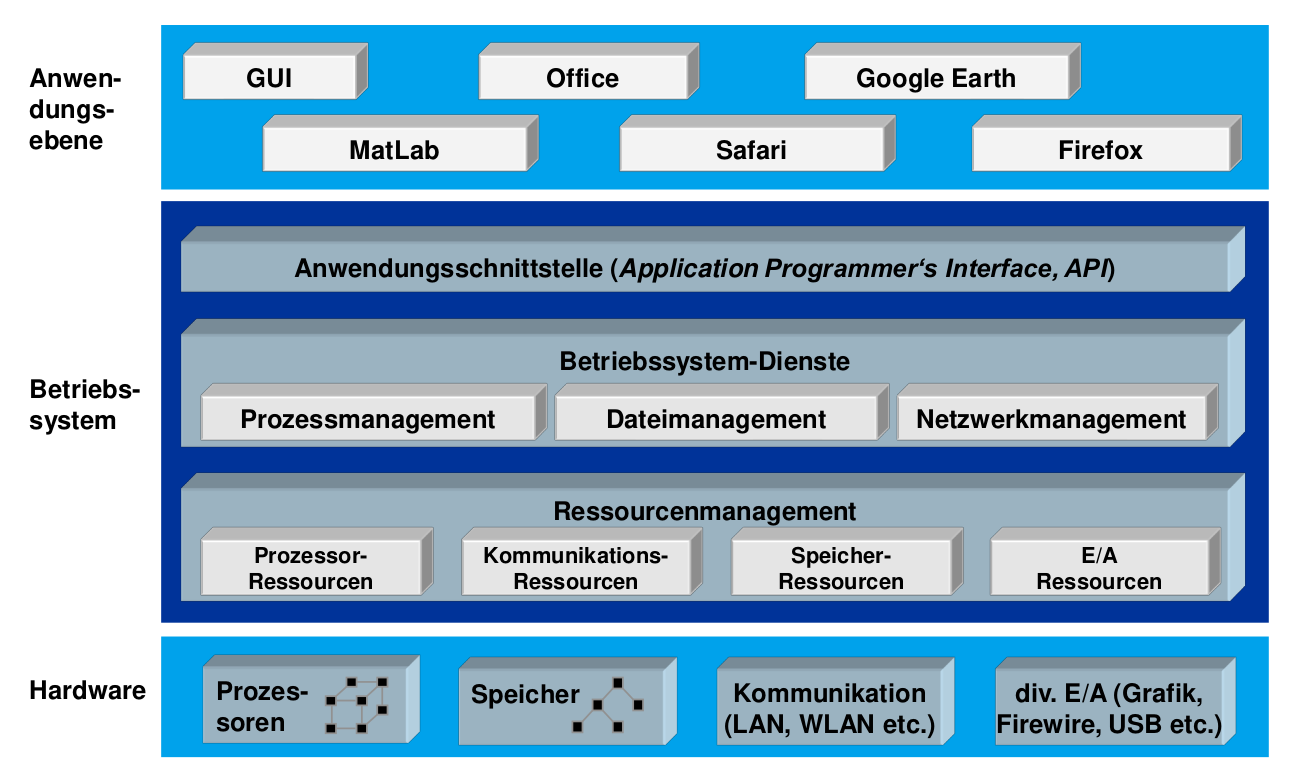
\includegraphics[width=\textwidth/4]{Assets/Betriebssysteme_Uebersicht.png}}

\paragraph{Prozesse}
\begin{itemize*}
    \item BS-Abstraktionen zur Ausführung von Programmen
    \item Eigentümer von Ressourcen
    \item differenzierte Prozessmodelle: definieren konkrete Prozesseigenschaften
\end{itemize*}

\section{Was sind Datenbanken - Grundlegende Konzepte}
\subsection{Überblick}
\begin{itemize*}
    \item Daten = logisch gruppierte Informationseinheiten
    \item Bank = Sicherheit vor Verlust, Dienstleistung für mehrere Kunden, (langfristige) Aufbewahrung
\end{itemize*}

Ohne Datenbanken:
\begin{itemize*}
    \item jedes Anwendungssystem verwaltet seine eigenen Daten
    \item Daten sind (redundant) mehrfach gespeichert
    \item Probleme
    \begin{itemize*}
        \item Verschwenden von Speicherplatz
        \item "vergessen" von Änderungen
        \item keine zentrale "genormte" Datenerhaltung
    \end{itemize*}
    \item größere Mengen von Daten nicht effizient verarbeitet
    \item mehrere Benutzer können nicht parallel auf den gleichen Daten arbeiten, ohne sich zu stören
    \item Anwendungsprogrammierer/Benutzer können Anwendungen nicht programmieren/benutzen ohne ... zu kennen (keine Datenunabhängigkeit)
    \begin{itemize*}
        \item interne Dartstellung der Daten
        \item Speichermedien oder Rechner
    \end{itemize*}
    \item Datenschutz und   Datensicherheit
\end{itemize*}

\paragraph{Datenintegration durch Datenbanksystem}
Anwendungen greifen über Datenbankmanagementsystem auf Datenbank zu.

Datenbankmanagementsystem (DBMS): Software zur Verwaltung von Datenbanken

Datenbank (DB): strukturierter, von DBMS verwalteter Datenbestand

Datenbanksystem (DBS) = DBMS + DB

\subsection{Architekturen}
die neun Codd"schen Regeln
\begin{enumerate*}
    \item Integration: einheitliche, nichtredundante Datenverwaltung
    \item Operationen: Speichern, Suchen, Ändern
    \item Katalog: Zugriffe auf Datenbankbeschreibungen im Data Dictionary
    \item Benutzersichten
    \item Integritätssicherung: Korrektheit des Datenbankinhalts
    \item Datenschutz: Ausschluss unauthorisierter Zugriffe
    \item Transaktionen: mehrere DB-Operationen als Funktionseinheit
    \item Synchronisation: parallele Transaktionen koordinieren
    \item Datensicherung: Wiederherstellung von Daten nach Systemfehlern
\end{enumerate*}

Ziele:
\begin{itemize*}
    \item Trennung von Modellierungssicht und interner Speicherung
    \item Portierbarkeit
    \item Tuning vereinfachen
    \item standardisierte Schnittstellen
\end{itemize*}

Schemata:
\begin{itemize*}
    \item Konzeptuelles Schema (Ergebnis der Dateidefinition)
    \item Internes Schema (Festlegung der Dateiorganisation und Zugriffspfade = Index)
    \item Externes Schema (Ergebnis der Sichtdefinition)
    \item Anwendungsprogramm (Ergebnis der Anwendungsprogrammierung)
    \item Trennung Schema-Instanz
    \begin{itemize*}
        \item Schema: Metadaten, Datenbeschreibung
        \item Instanz: Anwenderdaten, Datenbankzustand
    \end{itemize*}
\end{itemize*}

Datenunabhängigkeit:
\begin{itemize*}
    \item Stabilität der Benutzerschnittstelle gegen Änderungen
    \item physisch: Änderung der Dateiorganisation und Zugriffspfade haben keinen Einfluss auf das konzeptuelle Schema
    \item logisch: Änderung am konzeptuellen und gewissen externen Schemata haben keine Auswirkungen auf andere externe Schemata und Anwendungsprogramme
\end{itemize*}

Aufteilung der Funktionalitäten einer Anwendung
\begin{itemize*}
    \item Präsentation und Benutzerinteraktion
    \item Anwendungslogik („Business“-Logik)
    \item Datenmanagementfunktionen (Speichern, Anfragen, ...)
\end{itemize*}

Architektur von Datenbankanwendungen typischerweise auf Basis des Client-Server-Modells (Server=Datenbanksystem).

\paragraph{3 Schichten Architektur (ANSI-SPARC-Architektur) }
Klassifizierung der Komponenten
\begin{itemize*}
    \item Definitionskomponenten: Datendefinition, Dateiorganisation, Sichtdefinition
    \item Programmierkomponenten: DB-Programmierung mit eingebetteten DB-Operationen
    \item Benutzerkomponenten: Anwendungsprogramme, Anfrage und Update interaktiv
    \item Transformationskomponenten: Optimierer, Auswertung, Plattenzugriffssteuerung
    \item Data Dictionary (Datenwörterbuch): Aufnahme der Daten aus Definitionskomponenten, Versorgung der anderen Komponenten
\end{itemize*}

\paragraph{5 Schichten Architektur}
Verfeinerung der Transformation
\begin{itemize*}
    \item Datensystem: Übersetzung, Zugriffspfadwahl
    \item Zugriffssystem: Logische Zugriffspfade, Schemakatalog, Sortierung, Transaktionsverwaltung
    \item Speichersystem Speicherungsstrukturen, Zugriffspfadverwaltung, Sperrverwaltung, Logging, Recovery
    \item Pufferverwaltung: Systempufferverwaltung, Seitenersetzung, Seitenzuordnung
    \item Betriebssystem: Externspeicherverwaltung, Speicherzuordnung
\end{itemize*}

\subsection{Einsatzgebiete}
\begin{itemize*}
    \item Klassische Einsatzgebiete:
    \begin{itemize*}
        \item viele Objekte (15000 Bücher, 300 Benutzer, 100 Ausleihvorgänge pro Woche, ...)
        \item wenige Objekttypen (BUCH, BENUTZER, AUSLEIHUNG)
        \item etwa Buchhaltungssysteme, Auftragserfassungssysteme, Bibliothekssysteme, ...
    \end{itemize*}
    \item Aktuelle Anwendungen: E-Commerce, entscheidungsunterstützende Systeme (Data Warehouses, OLAP), NASA’s Earth Observation System (Petabyte-Datenbanken), Data Mining
\end{itemize*}

\subsection{Historisches}
\begin{itemize*}
    \item Wissensbanksysteme
    \begin{itemize*}
        \item Daten in Tabellenstrukturen
        \item Stark deklarative DML, integrierte Datenbankprogrammiersprache
    \end{itemize*}
    \item Objektorientierte Datenbanksysteme
    \begin{itemize*}
        \item Daten in komplexeren Objektstrukturen (Trennung Objekt und seine Daten)
        \item Deklarative oder navigierende DML
        \item Oft integrierte Datenbankprogrammiersprache
        \item Oft keine vollständige Ebenentrennung
    \end{itemize*}
\end{itemize*}

\begin{itemize*}
    \item Neue Hardwarearchitekturen
    \item Unterstützung für spezielle Anwendungen
    \item Datenstromverarbeitung: Online-Verarbeitung von Live-Daten, z.B. Börseninfos, Sensordaten, RFID-Daten, ...(StreamBase, MS StreamInsight, IBM Infosphere Streams)
    \item NoSQL-Datenbanken („Not only SQL“):
    \begin{itemize*}
        \item nicht-relationale Datenbanken, flexibles Schema (dokumentenzentriert)
        \item „leichtgewichtig“ durch Weglassen von SQL-Funktionalitäten wie Transaktionen, mächtige deklarative Anfragesprachen mit Verbunden etc.
        \item Beispiele: CouchDB, MongoDB, Cassandra, ...
    \end{itemize*}
\end{itemize*}


\section{Relationale Datenbanken - Daten als Tabellen}
\subsection{Relationen für tabellarische Daten}
Konzeptuell: Datenbank = Menge von Tabellen (= Relationen)

\begin{itemize*}
    \item „Tabellenkopf“: Relationenschema
    \item Eine Zeile der Tabelle: Tupel; Menge aller Einträge: Relation
    \item Eine Spaltenüberschrift: Attribut
    \item Ein Eintrag: Attributwert
\end{itemize*}

Integritätsbedingungen: Schlüssel
\begin{itemize*}
    \item Attribute einer Spalte identifizieren eindeutig gespeicherte Tupel: Schlüsseleigenschaft
    \item auch Attributkombinationen können Schlüssel sein!
    \item Schlüssel können durch Unterstreichen gekennzeichnet werden
    \item Schlüssel einer Tabelle können in einer anderen (oder derselben!) Tabelle als eindeutige Verweise genutzt werden: Fremdschlüssel
    \item ein Fremdschlüssel ist ein Schlüssel in einer „fremden“ Tabelle
\end{itemize*}

\subsection{SQL-Datendefinition}
\paragraph{CREATE table}
Wirkung dieses Kommandos ist sowohl
\begin{itemize*}
    \item die Ablage des Relationenschemas im Data Dictionary, als auch
    \item die Vorbereitung einer „leeren Basisrelation“ in der Datenbank
\end{itemize*}

\paragraph{DROP table}
komplettes Löschen einer Tabelle (Inhalt und Eintrag im Data
Dictionary)

\paragraph{Mögliche Wertebereiche in SQL}
\begin{itemize*}
    \item integer (oder auch integer4, int),
    \item smallint (oder auch integer2),
    \item float(p) (oder auch kurz float),
    \item decimal(p,q) und numeric(p,q) mit jeweils q Nachkommastellen,
    \item character(n) (oder kurz char(n), bei n = 1 auch char) für Zeichenketten (Strings) fester Länge n,
    \item character varying(n) (oder kurz varchar(n) für Strings variabler Länge bis zur Maximallänge n,
    \item bit(n) oder bit varying(n) analog für Bitfolgen, und
    \item date, time bzw. datetime für Datums-, Zeit- und kombinierte Datums-Zeit-Angaben
\end{itemize*}

\begin{itemize*}
    \item primary key kennzeichnet Spalte als Schlüsselattribut
    \item foreign key kennzeichnet Spalte als Fremdschlüssel
    \item not null schließt in bestimmten Spalten Nullwerte als Attributwerte aus
    \item null repräsentiert die Bedeutung „Wert unbekannt“, „Wert nicht anwendbar“ oder „Wert existiert nicht“, gehört aber zu keinem Wertebereich
    \item null kann in allen Spalten auftauchen, außer in Schlüsselattributen und den mit not null gekennzeichneten
\end{itemize*}


\subsection{Grundoperationen: Die Relationenalgebra}
\begin{itemize*}
    \item Anfrageoperationen auf Tabellen
    \begin{itemize*}
        \item Basisoperationen auf Tabellen, die die Berechnung von neuen Ergebnistabellen aus gespeicherten Datenbanktabellen erlauben
        \item Operationen werden zur sogenannten Relationenalgebra zusammengefasst
        \item Mathematik: Algebra ist definiert durch Wertebereich sowie darauf definierten Operationen
        \begin{itemize*}
            \item für Datenbankanfragen entsprechen die Inhalte der Datenbank den Werten, Operationen sind dagegen Funktionen zum Berechnen der Anfrageergebnisse
        \end{itemize*}
        \item Anfrageoperationen sind beliebig kombinierbar und bilden eine Algebra zum „Rechnen mit Tabellen“ – die Relationenalgebra
    \end{itemize*}
\end{itemize*}

\begin{itemize*}
    \item Selektion $\sigma$: Auswahl von Zeilen einer Tabelle anhand eines Selektionsprädikats
    \item Projektion $\pi$: Auswahl von Spalten durch Angabe einer Attributliste
    \begin{itemize*}
        \item Die Projektion entfernt doppelte Tupel
    \end{itemize*}
    \item Verbund $\bowtie$ (engl. join): verknüpft Tabellen über gleichbenannte Spalten, indem er jeweils zwei Tupel verschmilzt, falls sie dort gleiche Werte aufweisen
    \begin{itemize*}
        \item Tupel, die keinen Partner finden (dangling tuples), werden eliminiert
    \end{itemize*}
    \item Umbenennung $\beta$: Anpassung von Attributnamen mittels Umbenennung
    \item Vereinigung $r_1 \cup r_2$ von zwei Relationen $r_1$ und $r_2$:
    \begin{itemize*}
        \item Gesamtheit der beiden Tupelmengen
        \item Attributmengen beider Relationen müssen identisch sein
    \end{itemize*}
    \item Differenz $r_1 - r_2$ eliminiert die Tupel aus der ersten Relation, die auch in der zweiten Relation vorkommen
    \item Durchschnitt $r_1 \cap r_2$: ergibt die Tupel, die in beiden Relationen gemeinsam vorkommen
\end{itemize*}


\subsection{SQL als Anfragesprache}
```sql
SELECT farbe FROM weine WHERE Jahrgang = 2002
```
\begin{itemize*}
    \item SQL hat Multimengensemantik — Duplikate in Tabellen werden in SQL nicht automatisch unterdrückt!
    \begin{itemize*}
        \item Mengensemantik durch distinct
    \end{itemize*}
    \item Verknüpfung von Tabellen
    \begin{itemize*}
        \item Kreuzprodukt: "" select * from Weine, Erzeuger""
        \item Verbund: "" select * from Weine natural join Erzeuger""
        \item Verbund mit Bedingung: "" select * from Weine, Erzeuger where Weine.Weingut = Erzeuger.Weingut""
    \end{itemize*}
    \item Kombination von Bedingungen
    \item Vereinigung in SQL explizit mit union
\end{itemize*}

\subsection{Änderungsoperationen in SQL}
\begin{itemize*}
    \item insert: Einfügen eines oder mehrerer Tupel in eine Basisrelation oder Sicht
    \item update: Ändern von einem oder mehreren Tupel in einer Basisrelation oder Sicht
    \item delete: Löschen eines oder mehrerer Tupel aus einer Basisrelation oder Sicht
\end{itemize*}

Lokale und globale Integritätsbedingungen müssen bei Änderungsoperationen automatisch vom System überprüft werden


\section{Datenbankentwurf im ER-Modell}
\subsection{Datenbankmodelle}
> \textbf{Datenbankmodell}: Ein Datenbankmodell ist ein System von Konzepten zur Beschreibung von Datenbanken. Es legt Syntax und Semantik von Datenbankbeschreibungen für ein Datenbanksystem fest.

Datenbankbeschreibungen = Datenbankschemata

\begin{enumerate*}
    \item statische Eigenschaften
    \begin{itemize*}
        \item Objekte
        \item Beziehungen inklusive der Standard-Datentypen, die Daten über die Beziehungen und Objekte darstellen können,
    \end{itemize*}
    \item dynamische Eigenschaften wie
    \begin{itemize*}
        \item Operationen
        \item Beziehungen zwischen Operationen,
    \end{itemize*}
\end{enumerate*}

Datenbankmodelle im Überblick
\begin{itemize*}
    \item HM: hierarchisches Modell, NWM: Netzwerkmodell, RM: Relationenmodell
    \item NF 2 : Modell der geschachtelten (Non-First-Normal-Form = NF 2 ) Relationen, eNF 2 : erweitertes NF 2 -Modell
    \item ER: Entity-Relationship-Modell, SDM: semantische Datenmodelle
    \item OODM / C++: objektorientierte Datenmodelle auf Basis objektorientierter Programmiersprachen wie C++,
    \begin{itemize*}
        \item OEM: objektorientierte Entwurfsmodelle (etwa UML),
        \item ORDM: objektrelationale Datenmodelle
    \end{itemize*}
\end{itemize*}

\subsection{ER Modell}
\begin{itemize*}
    \item \textbf{Entity}: Objekt der realen oder der Vorstellungswelt, über das Informationen zu speichern sind, z.B. Produkte (Wein, Katalog), Winzer oder Kritiker; aber auch Informationen über Ereignisse, wie z.B. Bestellungen
    \item \textbf{Relationship}: beschreibt eine Beziehung zwischen Entities, z.B. ein Kunde bestellt einen Wein oder ein Wein wird von einem Winzer angeboten
    \item \textbf{Attribut}: repräsentiert eine Eigenschaft von Entities oder Beziehungen, z.B. Name eines Kunden, Farbe eines Weines oder Datum einer Bestellung
    \begin{itemize*}
        \item Attribute modellieren Eigenschaften von Entities oder auch Beziehungen
        \item alle Entities eines Entity-Typs haben dieselben Arten von Eigenschaften; Attribute werden somit für Entity-Typen deklariert
    \end{itemize*}
    \item \textbf{Werte}: primitive Datenelemente, die direkt darstellbar sind
    \begin{itemize*}
        \item Wertemengen sind beschrieben durch Datentypen, die neben einer Wertemenge auch die Grundoperationen auf diesen Werten charakterisieren
        \item ER-Modell: vorgegebene Standard-Datentypen, etwa die ganzen Zahlen int, die Zeichenketten string, Datumswerte date etc.
        \item jeder Datentyp stellt Wertebereich mit Operationen und Prädikaten dar
    \end{itemize*}
    \item \textbf{Entities} sind die in einer Datenbank zu repräsentierenden Informationseinheiten
    \begin{itemize*}
        \item im Gegensatz zu Werten nicht direkt darstellbar, sondern nur über ihre Eigenschaften beobachtbar
        \item Entities sind eingeteilt in Entity-Typen, etwa $E_1 , E_2,...$
    \end{itemize*}
    \item \textbf{Schlüsselattribute}: Teilmenge der gesamten Attribute eines Entity-Typs $E(A_1,... , A_m)$
    \begin{itemize*}
        \item in jedem Datenbankzustand identifizieren die aktuellen Werte der Schlüsselattribute eindeutig Instanzen des Entity-Typs E
        \item bei mehreren möglichen Schlüsselkandidaten: Auswahl eines Primärschlüssels
    \end{itemize*}
    \item \textbf{Beziehungstypen}: Beziehungen zwischen Entities werden zu Beziehungstypen zusammengefasst
    \begin{itemize*}
        \item Beziehungen können ebenfalls Attribute besitzen
    \end{itemize*}
\end{itemize*}


Merkmale von Beziehungen
\begin{itemize*}
    \item Stelligkeit oder Grad:
    \begin{itemize*}
        \item Anzahl der beteiligten Entity-Typen
        \item häufig: binär
        \item Beispiel: Lieferant liefert Produkt
    \end{itemize*}
    \item Kardinalität oder Funktionalität:
    \begin{itemize*}
        \item Anzahl der eingehenden Instanzen eines Entity-Typs
        \item Formen: 1:1, 1:n, m:n
        \item stellt Integritätsbedingung dar
        \item Beispiel: maximal 5 Produkte pro Bestellung
    \end{itemize*}
\end{itemize*}

\begin{itemize*}
    \item 1:1 Beziehung
    \begin{itemize*}
        \item jedem Entity $e_1$ vom Entity-Typ $E_1$ ist maximal ein Entity $e_2$ aus $E_2$ zugeordnet und umgekehrt
        \item Bsp: Prospekt *beschreibt* Produkt
    \end{itemize*}
    \item 1:N Beziehung
    \begin{itemize*}
        \item jedem Entity $e_1$ aus $E_1$ sind beliebig viele Entities $E_2$ zugeordnet, aber zu jedem Entity $e_2$ gibt es maximal ein $e_1$ aus $E_1$
        \item Bsp: Lieferant *liefert* Produkte, Mutter *hat* Kinder
    \end{itemize*}
    \item N:1 Beziehung
    \begin{itemize*}
        \item invers zu 1:N, auf funktionale Beziehung
    \end{itemize*}
    \item M:N Bezeihung
    \begin{itemize*}
        \item keine Restriktionen
        \item Bsp: Bestellung *umfasst* Produkte
    \end{itemize*}
\end{itemize*}

[min,max]-Notation
\begin{itemize*}
    \item schränkt die möglichen Teilnahmen von Instanzen der beteiligten Entity-Typen an der Beziehung ein, indem ein minimaler und ein maximaler Wert vorgegeben wird
    \item Spezielle Wertangabe für $max_i$ ist *
\end{itemize*}

Kardinalitätsangaben
\begin{itemize*}
    \item [0, *] legt keine Einschränkung fest (default)
    \item $R(E_1 [0, 1], E_2 )$ entspricht einer (partiellen) funktionalen Beziehung $R : E_1 \rightarrow E_2$ , da jede Instanz aus $E_1$ maximal einer Instanz aus $E_2$ zugeordnet ist
    \item totale funktionale Beziehung wird durch $R(E_1 [1, 1], E_2 )$ modelliert
    \item Beispiele:
    \begin{itemize*}
        \item partielle funktionale Beziehung: $lagert_in(Produkt[0,1],Fach[0,3])$
        \item totale funktionale Beziehung: $liefert(Lieferant[0,*],Produkt[1,1])$
    \end{itemize*}
\end{itemize*}

\subsection{Weitere Konzepte im ER Modell}
\begin{itemize*}
    \item abhängiger Entity-Typ: Identifikation über funktionale Beziehungen (Bsp x "gehört zu" y)
    \item Spezialisierungs-/Generalisierungsbeziehung oder auch *IST*-Beziehung
    \begin{itemize*}
        \item E1 *IST* E2
        \item entspricht semantisch einer injektiven funktionalen Beziehung
        \item Attribute des Entity-Typs E2 treffen auch auf E1 zu: "vererbte" Attribute
        \item nicht nur Atrributsdeklarationen vererben sich, sondern auch jeweils die aktuellen Werte für eine Instanz
        \item Kardinalitätsangabe immer: $IST(E_1[1,1], E_2[0,1])$
        \item Jede Instanz von E1 nimmt genau einmal an der Ist-Beziehung teil, während Instanzen des Obertyps E2 nicht teilnehmen müssen
    \end{itemize*}
\end{itemize*}

Die Konzepte im Überblick:
| Begriff | Informale Bedeutung |
| Entity | zu repräsentierende Informationseinheit |
| Entity Typ | Gruppierung von Entitys mit gleichen Eigenschaften |
| Beziehungstyp | Gruppierung von Beziehungen zwischen Entitys |
| Attribut | datenwertige Eigenschaft eines Entitys oder einer Beziehung |
| Schlüssel | identifizierende Eigenschaft von Entitys |
| Kardinalitäten | Einschränkung von Beziehungstypen bezüglich der mehrfachen Teilnahme von Entitys an der Beziehung |
| Stelligkeit | Anzahl der an einem Beziehungstyp beteiligten Entity Typen |
| funktionale Beziehungen | Beziehungstyp mit Funktionseigenschaften |
| abhängige Entitys | Entitys, die nur abhängig von anderen Entitys existieren können |
| IST Beziehung | Spezialisierung von Entity Typen |
| Optionalität | Attribute oder Funktionale Beziehungen als partielle Funktionen |


\section{Datenbankentwurf}
\subsection{Phasen des Datenbankentwurfs}
\begin{itemize*}
    \item Datenerhaltung für mehrere Anwendungssysteme und mehrere Jahre
    \item Anforderungen an Entwurf:
    \begin{itemize*}
        \item Anwendungsdaten jeder Anwendung sollen aus Daten der Datenbank ableitbar sein (mögl effizient)
        \item nur "vernünftige" Daten sollen gespeichert werden
        \item nicht-redundante Speicherung
    \end{itemize*}
\end{itemize*}

\paragraph{Phasenmodell}
Anforderungsanalyse $\leftrightarrow$ Konzeptioneller Entwurf  $\leftrightarrow$ Verteilungsentwurf $\leftrightarrow$ Logischer Entwurf $\leftrightarrow$ Datendefinition $\leftrightarrow$ Physischer Entwurf $\leftrightarrow$ Implementierung \& Wartung

\paragraph{Anforderungsanalyse}
\begin{itemize*}
    \item Vorgehensweise: Sammeln des Informationsbedarfs in den Fachabteilungen
    \item Ergebnis:
    \begin{itemize*}
        \item informale Beschreibung des Fachproblems (Texte, Tabellen, Formblätter,...)
        \item Trennen der Informationen über Daten (Datenanalyse) von den Informationen über Funktionen (Funktionsanalyse)
    \end{itemize*}
    \item "Klassischer" Entwurf: nur Datenanalyse und Folgeschritte
    \item Funktionsentwurf: siehe Methoden des Software Engineering
\end{itemize*}

\paragraph{Konzeptioneller Entwurf}
\begin{itemize*}
    \item erste Formale Beschreibung des Fachproblems
    \item Sprachmittel: semantisches Datenmodell
    \item Vorgehensweise:
    \begin{itemize*}
        \item Modellierung von Sichen z.B. für verschiedene Fachabteilungen
        \item Analyse der vorliegenden Sichten in Bezug auf Konflikte
        \item Integration der Sichten in ein Gesamtschema
    \end{itemize*}
    \item Phasen:
    \begin{itemize*}
        \item Sichtentwurf
        \item Sichtanalyse
        \item Sichtintegration
    \end{itemize*}
    \item Ergebnis: konzeptionelles Gesamtschema (z.B. ER Schema)
\end{itemize*}

\paragraph{weiteres Vorgehen beim Entwurf}
\begin{itemize*}
    \item ER-Modellierung von verschiedenen Sichten auf Gesamtinformation, z.B. für verschiedene Fachabteilungen eines Unternehmens -> konzeptueller Entwurf
    \item Verteilungsentwurf bei verteilter Speicherung
    \item Abbildung auf konkretes Implementierungsmodell -> logischer Entwurf
    \item Datendefinition, Implementierung und Wartung -> physischer Entwurf
\end{itemize*}

\paragraph{Sichtintegration}
\begin{itemize*}
    \item Analyse der vorliegenden Sichten in Bezug auf Konflikte
    \item Integration der Sichten in ein Gesamtschema
\end{itemize*}

\paragraph{Integrationskonflikte}
\begin{itemize*}
    \item Namenskonflikte: Homonyme/Synonyme
    \item Typkonflikte: verschiedene Strukturen für das gleiche Element
    \item Wertebereichskonflikte: verschiedene Wertebereiche für ein Element
    \item Bedingungskonflikte: z.B. verschiedene Schlüssel für ein Element
    \item Strukturkonflikte: gleicher Sachverhalt durch unterschiedliche Konstrukte ausgedrückt
\end{itemize*}

\paragraph{Verteilungsentwurf}
\begin{itemize*}
    \item sollen Daten auf mehreren Rechnern verteilt vorliegen, muss Art und Weise der verteilten Speicherung festgelegt werden
    \item horizontale Verteilung z.B. Kunden 1-1000 und Kunden 10001-20000
    \item vertikale Verteilung z.B. Adresse in DB1, Konto in DB2
\end{itemize*}

\paragraph{Logischer Entwurf}
\begin{itemize*}
    \item Sprachmittel: Datenmodell des ausgewählten "Realisierungs"DBMS
    \item Vorgehensweise
    \begin{enumerate*}
        \item (automatische) Transformation des konzeptionellen Schemas z.B. ER -> relationales Modell
        \item Verbesserung des relationalen Schemas anhand von Gütekriterien
    \end{enumerate*}
    \item Ergebnis: logisches Schema
\end{itemize*}

\paragraph{Datendefinition}
\begin{itemize*}
    \item Umsetzung des logischen Schemas in ein konkretes Schema
    \item Sprachmittel: DDL und DML eines DBMS
    \begin{itemize*}
        \item Datenbankdeklaration in der DDL des DBMS
        \item Realisierung der Integritätssicherung
        \item Definition der Benutzersichten
    \end{itemize*}
\end{itemize*}

\paragraph{Physischer Entwurf}
\begin{itemize*}
    \item Ergänzen des physischen Entwurfs um Zugriffsunterstützung bzgl Effizienzverbesserung, z.B. Definition von Indexen
    \item Index:
    \begin{itemize*}
        \item Zugriffspfad: Datenstruktur für zusätzlichen, schlüsselbasierten Zugriff auf Tupel
        \item meist als B*-Baum realisiert
    \end{itemize*}
    \item Sprachmittel: Speicherstruktursprache SSL
\end{itemize*}

Indexe in SQL, z.B.: ```create index WeinIdx on WEINE (Name)```

Notwendigkeit für Zugriffspfade:
\begin{itemize*}
    \item Beispiel: Tabelle mit 100GB Daten, Festplattentransferrate ca 50MB/s
    \item Operation: Suchen eines Tupels (Selektion)
    \item Implementierung: sequentielles Durchsuchen
    \item Aufwand: 102.500/50 = 2048 sec ~ 34 Minuten
\end{itemize*}

\paragraph{Implementierung \& Wartung}
\begin{itemize*}
    \item Wartung
    \item weitere Optimierung der physischen Ebene
    \item Anpassung an neue Anforderungen und Systemplattformen
    \item Portierung auf neue Datenbankmanagementsysteme
    \item etc
\end{itemize*}


\subsection{Kapazitätserhaltende Abbildungen}
Umsetzung des konzeptionellen Schemas
\begin{itemize*}
    \item Umsetzung auf logisches Schema
    \item Erhaltung der Informationskapazität
    \item Kapazitäts\textbf{erhöhende} Abbildung: Abbildung auf R mit genau einem Schlüssel K ( K={{A},{B}} )
    \item Kapazitäts\textbf{vermindernde} Abbildung: Relationsschema mit einem Schlüssel
    \item Kapazitäts\textbf{erhaltende} Abbildung: kapazitätserhaltend mit Schlüssel beider Entity Typen im Relationsschema als neuer Schlüssel
\end{itemize*}

\subsection{ER-auf-RM Abbildung}
\paragraph{ER Abbildung auf Relationen}
\begin{itemize*}
    \item Entity-Typen und Beziehungstypen: jeweils auf Relationenschemata
    \item Attribute: Attribute des Relationenschemas, Schlüssel werden übernommen
    \item Kardinalitäten der Beziehungen: durch Wahl der Schlüssel bei den zugehörigen Relationenschemata ausgedrückt
    \item in einigen Fällen: Verschmelzen der Relationenschemata von Entity- und Beziehungstypen
    \item zwischen den verbleibenden Relationenschemata diverse Fremdschlüsselbedingungen einführen
\end{itemize*}

\paragraph{Abbildung von Beziehungstypen}
\begin{itemize*}
    \item neues Relationenschema mit allen Attributen des Beziehungstyps, zusätzlich Übernahme aller Primärschlüssel der beteiligten Entity-Typen
    \item Festlegung der Schlüssel:
    \begin{itemize*}
        \item m:n-Beziehung: beide Primärschlüssel zusammen werden Schlüssel im neuen Relationenschema
        \item 1:n-Beziehung: Primärschlüssel der n-Seite (bei der funktionalen Notation die Seite ohne Pfeilspitze) wird Schlüssel im neuen Relationenschema
        \item 1:1-Beziehung: beide Primärschlüssel werden je ein Schlüssel im neuen Relationenschema, der Primärschlüssel wird dann aus diesen Schlüsseln gewählt
    \end{itemize*}
    \item optionale Beziehungen ([0,1] oder [0,n]) werden nicht verschmolzen
    \item bei Kardinalitäten [1,1] oder [1,n] (zwingende Beziehungen) Verschmelzung möglich:
    \begin{itemize*}
        \item 1:n-Beziehung: das Entity-Relationenschema der n-Seite kann in das Relationenschema der Beziehung integriert werden
        \item 1:1-Beziehung: beide Entity-Relationenschemata können in das Relationenschema der Beziehung integriert werden
    \end{itemize*}
\end{itemize*}

\subsection{Übersicht über Transformationen}
| ER Konzept | wird abgebildet auf relationales Konzept |
| Entity Typ $E_i$      | Relationsenschema $R_i$ |
| Attribute von $E_i$   | Attribute von $R_i$     |
| Primärschlüssel $P_i$ | Primärschlüssel $P_i$   |
| Beziehungstyp         | Relationenschema, Attribute $P_1,P_2$ |
| dessen Attribute      | weitere Attribute       |
| 1:n                   | $P_2$ wird Primärschlüssel der Beziehung |
| 1:1                   | $P_1$ und $P_2$ werden Schlüssel der Beziehung |
| m:n                   | $P_1 \cup P_2$ wird Primärschlüssel der Beziehung |
| IST Beziehung         | $R_1$ erhält zusätzlichen Schlüssel $P_2$ |

\section{Relationaler Entwurf}
\subsection{Zielmodell des logischen Entwurfs}

Begriffe des Relationenmodells
| Begriff | Informale Bedeutung |
| Attribut | Spalte einer Tabelle |
| Wertebereich | mögliche Werte eines Attributs (auch Domäne) |
| Attributwert | Element eines Wertebereichs |
| Relationenschema | Menge von Attributen |
| Relation | Menge von Zeilen einer Tabelle |
| Tupel | Zeile einer Tabelle |
| Datenbankschema | Menge von Relationenschemata |
| Datenbank | Menge von Relationen (Basisrelationen) |
| Schlüssel | minimale Menge von Attributen, deren Werte ein Tupel einer Tabelle eindeutig identifizieren |
| Primärschlüssel | ein beim Datenbankentwurf ausgezeichneter Schlüssel |
| Fremdschlüssel | Attributmenge, die in einer anderen Relation Schlüssel ist |
| Fremdschlüsselbedingung | alle Attributwerte des Fremdschlüssels tauchen in der anderen Relation als Werte des Schlüssels auf |

Formalisierung Relationenmodell
\begin{itemize*}
    \item Attribute und Domänen
    \begin{itemize*}
        \item $U$ nichtleere, endliche Menge: Universum
        \item $A\in U$: Attribut
        \item $D = {D_1,..., D_m}$ Menge endlicher, nichtleerer Mengen: jedes $D_i$: Wertebereich oder Domäne
        \item total definierte Funktion $dom:U \rightarrow D$
        \item $dom(A)$: Domäne von A
        \item $w \in dom(A)$: Attributwert für A
    \end{itemize*}
    \item Relationenschemata und Relationen
    \begin{itemize*}
        \item $R\subseteq U$: Relationenschema
        \item Relation $r$ über $R = {A_1,..., A_n}$ (kurz: $r(R)$) ist endliche Menge von Abbildungen $t:R \rightarrow \bigcup_{i=1}^{m} D_i$, Tupel genannt
        \item Es gilt $t(A) \in dom(A)$ ($t(A)$ Restriktion von $t$ auf $A \in R$)
        \item für $X\subseteq R$ analog $t(X)$ X-Wert von $t$
        \item Menge aller Relationen über $R: REL(R) := {r | r(R)}$
    \end{itemize*}
    \item Datenbankschema und Datenbank
    \begin{itemize*}
        \item Menge von Relationenschemata $S := {R_1,..., R_p }:$ Datenbankschema
        \item Datenbank über $S$: Menge von Relationen $d:={r_1,..., r_p}$, wobei $r_i (R_i)$
        \item Datenbank $d$ über $S: d(S)$
        \item Relation $r\in d$: Basisrelation
    \end{itemize*}

    Integritätsbedingung
    \begin{itemize*}
        \item Identifizierende Attributmenge $K:= {B_1,..., B_k } \subseteq R: \forall t_1, t_2 \in r [t_1 \not = t_2 \Rightarrow \exists B \in K: t_1(B) \not = t_2(B)]$
        \item Schlüssel: ist minimale identifizierende Attributmenge
        \item Primattribut: Element eines Schlüssels
        \item Primärschlüssel: ausgezeichneter Schlüssel
        \item Oberschlüssel oder Superkey: jede Obermenge eines Schlüssels (= identifizierende Attributmenge)
        \item Fremdschlüssel: $X(R_1)\rightarrow Y(R_2)$
    \end{itemize*}
\end{itemize*}


\subsection{Relationaler DB-Entwurf}
\textbf{Redundanzen} in Basisrelationen sind aus mehreren Gründen unerwünscht:
\begin{itemize*}
    \item Redundante Informationen belegen unnötigen Speicherplatz
    \item Änderungsoperationen auf Basisrelationen mit Redundanzen nur schwer korrekt umsetzbar:
    \begin{itemize*}
        \item wenn eine Information redundant vorkommt, muss eine Änderung diese Information in allen ihren Vorkommen verändern
        \item mit normalen relationalen Änderungsoperationen und den in
        \item relationalen Systemen vorkommenden lokalen
        \item Integritätsbedingungen (Schlüsseln) nur schwer realisierbar
    \end{itemize*}
\end{itemize*}

Funktionale Abhängigkeit zwischen Attributemengen X und Y
> Wenn in jedem Tupel der Relation der Attributwert unter den X-Komponenten den Attributwert unter den Y-Komponenten festlegt.
\begin{itemize*}
    \item Unterscheiden sich zwei Tupel in den X-Attributen nicht, so haben sie auch gleiche Werte für alle Y-Attribute
    \item Notation für funktionale Abhängigkeit (FD, von functional dependency): X $\rightarrow$ Y
\end{itemize*}

> Ziel des Datenbankentwurfs: alle gegebenen funktionalen Abhängigkeiten in Schlüsselabhängigkeiten umformen, ohne dabei semantische Information zu verlieren

\subsection{Normalformen}
Schemaeigenschaften
\begin{itemize*}
    \item Relationenschemata, Schlüssel und Fremdschlüssel so wählen, dass
    \begin{itemize*}
        \item alle Anwendungsdaten aus den Basisrelationen hergeleitet werden können,
        \item nur semantisch sinnvolle und konsistente Anwendungsdaten dargestellt werden können und
        \item die Anwendungsdaten möglichst nicht-redundant dargestellt werden.
    \end{itemize*}
    \item Hier: Forderung 3
    \begin{itemize*}
        \item Redundanzen innerhalb einer Relation: Normalformen
        \item globale Redundanzen: Minimalität
    \end{itemize*}
\end{itemize*}

Normalformen
\begin{itemize*}
    \item legen Eigenschaften von Relationenschemata fest
    \item verbieten bestimmte Kombinationen von funktionalen Abhängigkeiten in Relationen
    \item sollen Redundanzen und Anomalien vermeiden
\end{itemize*}

\begin{enumerate*}
    \item Erste Normalform
    \begin{itemize*}
        \item erlaubt nur atomare Attribute in den Relationenschemata, d.h. als Attributwerte sind Elemente von Standard-Datentypen wie integer oder string erlaubt, aber keine Konstruktoren wie array oder set
    \end{itemize*}
    \item Zweite Normalform
    \begin{itemize*}
        \item Zweite Normalform eliminiert derartige partielle Abhängigkeiten bei Nichtschlüsselattributen
        \item partielle Abhängigkeit liegt vor, wenn ein Attribut funktional schon von einem Teil des Schlüssels abhängt
        \item Beispielrelation in 2 NF
        \begin{itemize*}
            \item R1(Name, Weingut, Preis)
            \item R2(Name, Farbe)
            \item R3(Weingut, Anbaugebiet, Region)
        \end{itemize*}
    \end{itemize*}
    \item Dritte Normalform
    \begin{itemize*}
        \item eliminiert (zusätzlich) transitive Abhängigkeiten
        \item etwa Weingut $\rightarrow$ Anbaugebiet und Anbaugebiet $\rightarrow$ Region in Relation
        \item man beachte: 3 NF betrachtet nur Nicht-Schlüsselattribute als Endpunkt transitiver Abhängigkeiten
        \item Beispielrelation in 3NF, transitive Abhängigkeit in R3, d.h. R3 verletzt 3NF
    \end{itemize*}
\end{enumerate*}

Dritte Normalform:
$A \in R$ heißt transitiv abhängig von X bezüglich F genau dann, wenn es ein $Y\subseteq R$ gibt mit $X \rightarrow Y, Y \not\rightarrow X, Y \rightarrow A, A \not\in XY$
\begin{itemize*}
    \item erweitertes Relationenschema $R=(R, \bf{K})$ ist in 3 NF bezüglich F genau dann, wenn $\not\exists A \in R$:
    \item A ist Nicht-Primattribut in R
    \item $\wedge A$ transitiv abhängig von einem $K\in \bf{K}$ bezüglich $F_i$.
    \item Nicht-Primattribut: A ist in keinem Schlüssel von R enthalten
\end{itemize*}

Boyce-Kodd-Normalform (Verschärfung der 3NF): Eliminierung transitiver Abhängigkeiten auch zwischen Primattributen $\not\exists A \in R$: A transitiv abhängig von einem $K\in\bf{K}$ bezüglich F

Minimalität
\begin{itemize*}
    \item Global Redundanzen vermeiden
    \item andere Kriterien (wie Normalformen) mit möglichst wenig Schemata erreichen
    \item Beispiel: Attributmenge ABC, FD-Menge ${A \rightarrow B, B \rightarrow C}$
\end{itemize*}

Übersicht
| Kennung | Schemaeigenschaft | Kurzcharakteristik |
| | 1 NF | nur atomare Attribute |
| | 2 NF | keine partielle Abhängigkeit eines Nicht-Primattributes von einem Schlüssel |
| S1 | 3 NF | keine transitive Abhängigkeit eines Nicht-Primattributs von einem Schlüssel |
| | BCNF | keine transitive Abhängigkei eines Attributes von einem Schlüssel |
| S2 | Minimalität | minimale Anzahl von Relationsschemata, die die anderen Eigenschaften erfüllt |

\subsection{Transformationseigenschaften}
\begin{itemize*}
    \item bei einer Zerlegung einer Relation in mehrere Relationen ist darauf zu achten, dass
    \begin{itemize*}
        \item nur semantisch sinvolle und konsistente Anwendungsdaten dargestellt (Abhängigkeitstreue) und
        \item alle Anwendungsdaten aus den Basisrelationen hergeleitet werden können (Verbundtreue)
    \end{itemize*}
    \item Abhänggikeitstreue (Kennung T1)
    \begin{itemize*}
        \item alle gegebenen Abhängigkeiten sind durch Schlüssel repräsentiert
        \item eine Menge von Abhängigkeiten kann äquivalent in eine zweite Menge von Abhängigkeiten transformiert werden
        \item spezieller: in die Menge der Schlüsselabhängigkeiten, da diese vom Datenbanksystem effizient überprüft werden kann
        \item die Menge der Abhängigkeiten soll äquivalent zu der Menge der Schlüsselbedingungen im resultierenden Datenbankschema sein
        \item Äquivalenz sichert zu, dass mit den Schlüsselabhängigkeiten semantisch genau die gleichen Integritätsbedingungen ausgedrückt werden wie mit den funktionalen oder anderen Abhängigkeiten vorher
        \item S charakterisiert vollständig F (oder: ist abhängigkeitstreu bezüglich F) genau dann, wenn $F\equiv \{K\rightarrow R | (R,\bf{K})\in S, K\in\bf{K}\}$
    \end{itemize*}
    \item Verbundtreue (Kennung T2)
    \begin{itemize*}
        \item Originalrelationen können durch den Verbund der Basisrelationen wiedergewonnen werden
        \item zur Erfüllung des Kriteriums der Normalformen müssen Relationenschemata teilweise in kleinere Relationenschemata zerlegt werden
        \item für Beschränkung auf „sinnvolle“ Zerlegungen gilt Forderung, dass die Originalrelation wieder aus den zerlegten Relationen mit dem natürlichen Verbund zurückgewonnen werden kann
        \item Zerlegung des Relationenschemas $R = ABC$ in $R_1 = AB$ und $R_2 = BC$
        \item Dekomposition bei Vorliegen der Abhängigkeiten $F = \{A \rightarrow B, C \rightarrow B\}$ ist nicht verbundtreu
        \item dagegen bei Vorliegen von $F" = \{A \rightarrow B, B \rightarrow C\}$ verbundtreu
    \end{itemize*}
\end{itemize*}

> Verbundtreue: Die Dekomposition einer Attributmenge $X$ in $X_1,..., X_p$ mit $X = \bigcup_{i=1}^p X_i$ heißt verbundtreu ($\pi \bowtie$-treu, lossless) bezüglich einer Menge von Abhängigkeiten F über X genau dann, wenn $\forall r \in SAT_X(F): \pi_{X_1}(r) \bowtie ... \bowtie \pi_{X_p}(r) = r$ gilt.

\subsection{Weitere Abhängigkeiten}
\begin{itemize*}
    \item Mehrwertige Abhängigkeit (kurz: MVD)
    \begin{itemize*}
        \item innerhalb einer Relation r wird einem Attributwert von X eine Menge von Y-Werten zugeordnet, unabhängig von den Werten der restlichen Attribute $\rightarrow$ Vierte Normalform
        \item Folge der 1NF: Mehrwertige Abhängigkeiten erzeugen Redundanz
        \item eine (oder mehrere) Gruppe von Attributwerten ist von einem Schlüssel bestimmt, unabhängig von anderen Attributen
        \item Resultat: Redundanz durch Bildung aller Kombinationen
        \item wünschenswerte Schemaeigenschaft bei Vorliegen von MVDs: vierte Normalform
        \item fordert die Beseitigung derartiger Redundanzen: keine zwei MVDs zwischen Attributen einer Relation
        \item Elimination der rechten Seite einer der beiden mehrwertigen Abhängigkeiten,
        \item linke Seite mit dieser rechten Seite in neue Relation kopiert
        \item Verbundabhängigkeit (kurz: JD)
        \item R kann ohne Informationsverlust in $R_1,..., R_p$ aufgetrennt werden: $\bowtie [R_1,..., R_p]$
        \item Inklusionsabhängigkeit (kurz: IND)
        \item auf der rechten Seite einer Fremdschlüsselabhängigkeit nicht unbedingt der Primärschlüssel einer Relation
    \end{itemize*}
\end{itemize*}

Vierte Normalform: erweitertes Relationenschema $R = (R, \bf{K})$ ist in vierter Normalform (4NF) bezüglich M genau dann, wenn für alle $X\rightarrow\rightarrow Y \in M^+$ gilt: $X\rightarrow\rightarrow Y$ ist trivial oder $X\supseteq K$ für ein $K\in\bf{K}$


\section{Relationale Theorie}
\subsection{Rechnen mit FDs}
\begin{itemize*}
    \item gilt für f über R $SAT_R(F)\subseteq SAT_R(f)$, dann impliziert F die FD f (kurz: $F\vdash f$)
    \item Hüllenbildung: Ermittlung aller funktionalen Abhängigkeiten, die aus einer gegebenen $FD_Menge$ abgeleitet werden können
    \item Hülle: $F_R^+ := \{ f | (f \text{ FD ueber R} ) \wedge F \vdash f\}$
\end{itemize*}

Ableitungsregel:
\begin{itemize*}
    \item F1: Reflexivität $X\supseteq Y \Rightarrow X\rightarrow Y$
    \item F2: Augumentation $\{X\rightarrow Y\}\Rightarrow XZ\rightarrow YZ, \text{ sowie } XZ\rightarrow Y$
    \item F3: Transitivität $\{ X\rightarrow Y,Y\rightarrow Z\}\Rightarrow X\rightarrow Y$
    \item F4: Dekomposition $\{X\rightarrow YZ\} \Rightarrow X\rightarrow Y$
    \item F5: Vereinigung $\{X\rightarrow Y, X\rightarrow Z\}\Rightarrow X\rightarrow YZ$
    \item F6: Pseudotransitivität $\{X\rightarrow Y, WY\rightarrow Z\}\Rightarrow WX\rightarrow Z$
\end{itemize*}

F1-F3 bekannt als Armstrong-Axiome (sound, complete)
\begin{itemize*}
    \item gültig (sound): Regeln leiten keine FDs ab, die logisch nicht impliziert
    \item vollständig (complete): alle implizierten FDs werden abgeleitet
    \item unabhängig (independent) oder  auch bzgl. $\subseteq$ minimal: keine Regel kann weggelassen werden
\end{itemize*}

Alternative Regelmenge
\begin{itemize*}
    \item B-Axiome oder RAP-Regeln
    \begin{itemize*}
        \item R Reflexivität $\{\}\Rightarrow X\rightarrow X$
        \item A Akkumulation $\{X\rightarrow YZ, Z\rightarrow AW\}\Rightarrow X\rightarrow YZA$
        \item P Projektivität $\{X\rightarrow YZ\}\Rightarrow X\rightarrow Y$
    \end{itemize*}
    \item Regelmenge ist vollständig, da Armstrong-Axiome daraus abgeleitet werden können
\end{itemize*}

> Membership Problem: Kann eine bestimmte FD $X\rightarrow Y$ aus der vorgegebenen Menge F abgeleitet werden, d.h. wird sie von F impliziert? $X\rightarrow Y \in F^+$
\begin{itemize*}
    \item Hülle einer Attributmenge X bzgl. F ist $X^+_F := \{A | X\rightarrow A \in F^+\}$
    \item Membership-Problem kann durch das modifizierte Problem $Y\subseteq X_F^+$ in linearer Zeit gelöst werden
\end{itemize*}

Überdeckungen
\begin{itemize*}
    \item F heißt äquivalent zu G; oder
    \item F Überdeckung von G; kurz: $F\equiv G$ falls $F^+=G^+$
    \item verschiedene Formen von Überdeckung: nicht-redundant, reduziert, minimal, ringförmig
\end{itemize*}

Reduktionsoperationen
\begin{itemize*}
    \item Ziel: Entfernen überflüssiger Attribute auf linker bzw. rechter Seite von FDs
    \item Linksreduktion: entfernt unwesentliche Attribute auf der linken Seite einer FD
    \item Rechtsreduktion: entsprechend auf der rechten Seite
    \item erw. Relationenschema $R = (R, K)$, FD-Menge F über R, A ist ein Attribut aus R und $X\rightarrow Y$ eine FD aus F
\end{itemize*}

Unwesentliche Attribute: A heißt unwesentlich in $X\rightarrow Y$ bzgl. F, wenn
\begin{itemize*}
    \item $X=AZ,Z\not= X \Rightarrow (F-\{X\rightarrow Y\})\cup \{Z\rightarrow Y\} \equiv F$ oder
    \item $Y=AW, W\not=Y\Rightarrow (F-\{X\rightarrow Y\})\cup \{X\rightarrow W\} \equiv F$
\end{itemize*}
\begin{itemize*}
    \item A kann also aus der FD $X\rightarrow Y$ entfernt werden, ohne dass sich die Hülle von F ändert
    \item FD $X\rightarrow Y$ heißt linksreduziert, wenn kein Attribut in X unwesentlich ist
    \item FD $X\rightarrow Y$ heißt rechtsreduziert, wenn kein Attribut in Y unwesentlich ist
\end{itemize*}

Minimale Überdeckung
\begin{itemize*}
    \item Eine minimale Überdeckung ist eine Überdeckung, die eine minimale Anzahl von FDs enthält
    \item Auswahl der kleinsten aller nicht-redundanten Überdeckungen
    \item FD-Menge F heißt minimal gdw. $\forall F" [F"\equiv \Rightarrow |F|\leq |F"|]$
    \item Bestimmung etwa durch reduzierte Überdeckung mit anschließender Äquivalenzklassenbildung (später)
\end{itemize*}

Äquivalenzklassen
\begin{itemize*}
    \item FDs mit äquivalenten linken Seiten werden zu einer Äquivalenzklasse zusammengefasst
    \item FDs $X_1 \rightarrow Y_1$ und $X_2\rightarrow Y_2$ liegen in einer Äquivalenzklasse, wenn $X_1\rightarrow X_2$ und $X_2\rightarrow X_1$ gelten
    \item In einigen Fällen können nun zwei solche FDs in einer Äquivalenzklasse zu einer FD $X\rightarrow Y_1 Y_2$ zusammengefasst werden
    \item Da die FDs einer Äquivalenzklasse in die Form $X_1\rightarrow X_2, X_2\rightarrow X_3,..., X_n\rightarrow X_1, X_1\rightarrow Y$ überführt werden können, nennt man eine Überdeckung dieser Form eine ringförmige Überdeckung
    \item linke Seiten sind äquivalent, wenn sie sich gegenseitig funktional bestimmen
\end{itemize*}


\subsection{Mehr zu Normalformen}
\begin{itemize*}
    \item partielle Abhängigkeit liegt vor, wenn ein Attribut funktional schon von einem Teil des Schlüssels abhängt
    \item Hinweis: partiell abhängiges Attribut stören nur, wenn es kein Primattribut ist
    \item 2NF formal: erweitertes Relationenschema $R = (R, K)$, FD-Menge F über R
\end{itemize*}

Zweite Normalform
\begin{itemize*}
    \item Y hängt partiell von X bzgl. F ab, wenn die FD $X\rightarrow Y$ nicht linksreduziert ist
    \item Y hängt voll von X ab, wenn die FD $X\rightarrow Y$ linksreduziert ist
    \item R ist in 2NF, wenn R in 1NF ist und jedes Nicht-Primattribut von R voll von jedem Schlüssel von R abhäng
\end{itemize*}

\subsection{Entwurfsverfahren}
Ziele:
\begin{itemize*}
    \item Universum $U$ und FD-Menge F gegeben
    \item lokal erweitertes Datenbankschema $S=\{(R_1, K_1),...,(R_p, K_p)\}$ berechnen mit
    \begin{itemize*}
        \item T1: S charakterisiert vollständig F
        \item S1: S ist in 3NF bezüglich F
        \item T2: Dekomosition von $U$ in $R_1,...,R_p$ ist verbundtreu bezüglich F
        \item S2: Minimalität, d.h. $\not\exists S":S"$ erfüllt T1,S1,T2 und $|S"|<|S|$
    \end{itemize*}
\end{itemize*}

Dekomposition:
\begin{itemize*}
    \item Geg.: initiales Universalrelationenschema $R = (U, K(F))$ mit allen Attributen und einer von erfassten FDs F über R implizierten Schlüsselmenge
    \begin{itemize*}
        \item Attributmenge U und eine FD-Menge F
        \item suche alle $K\rightarrow U$ mit K minimal, für die $K\rightarrow U \in F^+$ gilt $(K(F))$
    \end{itemize*}
    \item Ges.: Zerlegung in $D = \{R_1, R_2,... \}$ von 3NF-Relationenschemata
    \item Beispiel:
    \begin{itemize*}
        \item initiales Relationenschema $R=ABC$
        \item funktionale Abhängigkeiten $F=\{A\rightarrow B, B\rightarrow C\}$
        \item Schlüssel $K=A$
    \end{itemize*}
    \item Bewertung
    \begin{itemize*}
        \item Vorteile: 3NF, Verbundtreue
        \item Nachteile: restliche Kriterien nicht, reihenfolgeabhängig, NP-vollständig (Schlüsselsuche)
    \end{itemize*}
\end{itemize*}

Details zum Syntheseverfahren
\begin{itemize*}
    \item Prinzip: Synthese formt Original-FD-Menge F in resultierende Menge von Schlüsselabhängigkeiten G so um, dass $F\equiv G$ gilt
    \item „Abhängigkeitstreue“ im Verfahren verankert
    \item 3NF und Minimalität wird auch erreicht, reihenfolgeunabhängig
    \item Zeitkomplexität: quadratisch
\end{itemize*}

Syntheseverfahren für Relationenschema R mit FDs F
\begin{itemize*}
    \item Ges.: verlustfreie und abhängigkeitstreue Zerlegung in $R_1,... R_n$, wobei alle $R_i$ in 3NF sind
    \item Bilde Äquivalentklassen $C_i$ von FD aus $\hat{F}$ mit gleichen oder äquivalenten linken Seiten, d.h. $C_i=\{X_i\rightarrow A_{i1},X_i\rightarrow A_{i2},...\}$. Bilde zu jeder Äquivalenzklasse $C_i$ ein Schema der Form $R_{Ci}=\{X_i\cup \{A_{i1}\}\cup \{A_{i2}\}\cup ... \}$. Falls keines der Schemata $R_{Ci}$ enthält einen Schlüssel von R, erzeuge weiteres Relationenschema $R_K$ mit Attributen aus R, die Schlüssel bilden
    \item Beispiel
    \begin{itemize*}
        \item FD-Menge $F=\{A\rightarrow B, AB\rightarrow C, A\rightarrow C, B\rightarrow A, C\rightarrow E\}$
        \item minimale Überdeckung $\hat{F}=\{A\rightarrow B,B\rightarrow C, B\rightarrow A, C\rightarrow E\}$
        \item Zusammenfassung zu Äquivalenzklassen $C_1=\{A\rightarrow B,B\rightarrow C, B\rightarrow A\}, C_2=\{C\rightarrow E\}$
        \item Syntheseergebnis: $(ABC,\{\{A\},\{B\}\}),(CE,\{C\})$
    \end{itemize*}
\end{itemize*}

Erreichung der Verbundtreue
\begin{itemize*}
    \item Erreichen der Verbundtreue durch einfachen „Trick“:
    \begin{itemize*}
        \item Erweitern der Original-FD-Menge F um $U\rightarrow \delta$ um Dummy-Attribut $\delta$
        \item $\delta$ wird nach Synthese entfernt
    \end{itemize*}
    \item Beispiel: $\{A\rightarrow B, C\rightarrow E\}$
    \begin{itemize*}
        \item Syntheseergebnis $(AB, \{A\}), (CE, \{C\})$ ist nicht verbundtreu, da Universalschlüssel in keinem Schema enthalten ist
        \item Dummy-FD $ABCE\rightarrow \delta$; reduziert auf $AC\rightarrow\delta$
        \item liefert drittes Relationenschema $(AC,\{AC\})$
    \end{itemize*}
\end{itemize*}


\section{Die relationale Anfragesprache SQL}
\subsection{Aufbau von SQL-Anfragen}
\begin{itemize*}
    \item "select"
    \begin{itemize*}
        \item Projektionsliste
        \item Festlegung der Projektionsattribute
        \item arithmetische Operationen und Aggregatfunktionen
        \item Attribute der hinter from stehenden Relationen, optional mit Präfix, der Relationennamen oder Namen der Tupelvariablen angibt
        \item arithmetische Ausdrücke über Attributen dieser Relationen und passenden Konstanten
        \item Aggregatfunktionen über Attributen dieser Relationen
        \item Spezialfall der Projektionsliste: * ,liefert alle Attribute der Relation(en) aus dem from-Teil
        \item distinct eliminiert Duplikate
    \end{itemize*}
    \item "from"
    \begin{itemize*}
        \item zu verwendende Relationen, evtl. Umbenennungen
        \item einfachste Form; hinter jedem Relationennamen kann optional eine Tupelvariable stehen
    \end{itemize*}
    \item "where"
    \begin{itemize*}
        \item Selektions-, Verbundbedingungen
        \item Geschachtelte Anfragen (wieder ein SFW-Block)
    \end{itemize*}
\end{itemize*}

\paragraph{Verbunde}
\begin{itemize*}
    \item bei mehr als einer Relation wird das kartesische Produkt gebildet:
    "select * from WEINE, ERZEUGER"
    \item alle Kombinationen werden ausgegeben!
    \item Einführung von Tupelvariablen erlaubt mehrfachen Zugriff auf eine Relation:
    "select * from WEINE w1, WEINE w2"
    \begin{itemize*}
        \item Spalten lauten dann:
        "w1.WeinID, w1.Name, w1.Farbe, w1.Jahrgang, w1.Weingut, w2.WeinID, w2.Name, w2.Farbe, w2.Jahrgang, w2.Weingut"
    \end{itemize*}
    \item Natürlicher Verbund in SQL92
    "select * from WEINE, ERZEUGER where WEINE.Weingut = ERZEUGER.Weingut"
    \item Verbund mit "join"; kennen mehrere explizite Verbundoperatoren (engl. join);  als Abkürzung für die ausführliche Anfrage mit Kreuzprodukt aufzufassen
    "select * from WEINE natural join ERZEUGER"
    \begin{itemize*}
        \item Verbund mit beliebigem Prädikat: "select * from WEINE join ERZEUGER on WEINE.Weingut = ERZEUGER.Weingut"
        \item Gleichverbund mit using: "select * from WEINE join ERZEUGER using (Weingut)"
    \end{itemize*}
    \item Kreuzprodukt "select * from WEINE, ERZEUGER"
    \item als cross join "select * from WEINE cross join ERZEUGER"
    \item "Zwischenrelationen" aus SQL-Operationen oder einem SFW-Block können über Tupelvariablen mit Namen versehen werden
    "select Ergebnis.Weingut from (WEINE natural join ERZEUGER) as Ergebnis"
    \item Präfixe für Eindeutigkeit "select Name, Jahrgang, ERZEUGER.Weingut from WEINE natural join ERZEUGER"
    \item bei der Verwendung von Tupelvariablen, kann der Name einer Tupelvariablen zur Qualifizierung eines Attributs benutzt werden:
    "select w1.Name, w2.Weingut from WEINE w1, WEINE w2"
\end{itemize*}

\paragraph{Selektionen}
\begin{itemize*}
    \item where Klausel: "select ...from ... where bedingung"
    \begin{itemize*}
        \item Formen der Bedingung:
        \begin{itemize*}
            \item Vergleich eines Attributs mit einer Konstanten: "attribut $\Theta$ konstante"
            \item mögliche Vergleichssymbole $\Theta$ abhängig vom Wertebereich; etwa =, <>, >, <, >= sowie <=.
            \item Vergleich zwischen zwei Attributen mit kompatiblen Wertebereichen: "attribut1 $\Theta$ attribut2"
            \item logische Konnektoren or, and und not
        \end{itemize*}
    \end{itemize*}
    \item Verbundbedingung
    \begin{itemize*}
        \item Verbundbedingung hat die Form: "relation1.attribut = relation2.attribut"
        \item Beispiel: "select Name, Jahrgang, ERZEUGER.Weingut from WEINE, ERZEUGER where WEINE.Weingut = ERZEUGER.Weingut"
    \end{itemize*}
    \item Bereichsselektion
    \begin{itemize*}
        \item $attrib between konstante_1 and konstante_2$
        \item ist Abkürzung für $attrib \geq konstante_1$ and $attrib \leq konstante_2$
        \item schränkt damit Attributwerte auf das abgeschlossene Intervall $[konstante_1 , konstante_2 ]$ ein
        \item Beispiel: "select * from WEINE where Jahrgang between 2000 and 2005"
    \end{itemize*}
    \item Ungewissheitsselektion
    \begin{itemize*}
        \item Notation "attribut like spezialkonstante"
        \item Mustererkennung in Strings (Suche nach mehreren Teilzeichenketten)
        \item Spezialkonstante kann die Sondersymbole $\%$ und $\_$ beinhalten
        \begin{itemize*}
            \item \% steht für kein oder beliebig viele Zeichen
            \item $\_$ steht für genau ein Zeichen
        \end{itemize*}
        \item Beispiel: "select * from WEINE where Name like "La Rose\%""
    \end{itemize*}
\end{itemize*}

\paragraph{Mengenoperationen}
Mengenoperationen erfordern kompatible Wertebereiche für Paare korrespondierender Attribute:
\begin{itemize*}
    \item beide Wertebereiche sind gleich oder
    \item beide sind auf character basierende Wertebereiche (unabhängig von der Länge der Strings) oder
    \item beide sind numerische Wertebereiche (unabhängig von dem genauen Typ) wie integer oder float
    \item Ergebnisschema := Schema der „linken“ Relation
    ```sql
    select A, B, C from R1
    union
    select A, C, D from R2
    ```
\end{itemize*}

\begin{itemize*}
    \item Vereinigung, Durchschnitt und Differenz als union, intersect und except
    \item orthogonal einsetzbar:
    \item "select * from (select Weingut from ERZEUGER except select Weingut from WEINE)"
    \item äquivalent zu "select * from ERZEUGER except corresponding WEINE"
    \item über corresponding by-Klausel: Angabe der Attributliste, über die Mengenoperation ausgeführt wird
    \item "select * from ERZEUGER except corresponding by (Weingut) WEINE"
    \item bei Vereinigung: Defaultfall ist Duplikateliminierung (union distinct); ohne Duplikateliminierung durch union all
\end{itemize*}

\paragraph{Geschachtelte Anfragen}
Schachtelung von Anfragen
\begin{itemize*}
    \item für Vergleiche mit Wertemengen notwendig:
    \item Standardvergleiche in Verbindung mit den Quantoren all ($\forall$) oder any ($\exists$)
    \item spezielle Prädikate für den Zugriff auf Mengen, in und exists
    \item in-Prädikat und geschachtelte Anfragen
    \begin{itemize*}
        \item Notation: "attribut in ( SFW-block )"
        \item Beispiel: "select Name from WEINE where Weingut in (select Weingut from ERZEUGER where Region = "Bordeaux")"
        \item Auswertung von geschachtelten Anfragen
        \begin{itemize*}
            \item Auswertung der inneren Anfrage zu den Weingütern aus Bordeaux
            \item Einsetzen des Ergebnisses als Menge von Konstanten in die äußere Anfrage hinter in
            \item Auswertung der modifizierten Anfrage "select Name from WEINE where Weingut in ( "Château La Rose", "Château La Pointe")"
        \end{itemize*}
        \item interne Auswertung: Umformung in einen Verbund
        "select Name from WEINE natural join ERZEUGER where Region = "Bordeaux""
    \end{itemize*}
    \item Negation des in-Prädikats
    \begin{itemize*}
        \item Simulation des Differenzoperators $^\pi Weingut^{(ERZEUGER)}- ^\pi Weingut^{(WEINE)}$ durch SQL-Anfrage "select Weingut from ERZEUGER where Weingut not in ( select Weingut from WEINE )"
    \end{itemize*}
\end{itemize*}


\paragraph{Mächtigkeit des SQL-Kerns}
| Relationenalgebra  | SQL |
| Projektion | select distinct |
| Selektion | where ohne Schachtelung |
| Verbund | from, where\\ from mit join oder natural join |
| Umbenennung | from mit Tupelvariable; as |
| Differenz | where mit Schachtelung\\ except corresponding |
| Durchschnitt | where mit Schachtelung\\ intersect corresponding |
| Vereinigung | union corresponding |

\subsection{Erweiterungen des SFW-Blocks}
Erweiterungen des SFW-Blocks
\begin{itemize*}
    \item innerhalb der from-Klausel weitere Verbundoperationen (äußerer Verbund),
    \item innerhalb der where-Klausel weitere Arten von Bedingungen und Bedingungen mit Quantoren,
    \item innerhalb der select-Klausel die Anwendung von skalaren Operationen und Aggregatfunktionen,
    \item zusätzliche Klauseln group by und having
    \item rekursive Anfragen
\end{itemize*}

\paragraph{Skalare Ausdrücke}
Umbenennung von Spalten: "ausdruck as neuer-name"
\begin{itemize*}
    \item skalare Operationen auf
    \begin{itemize*}
        \item numerischen Wertebereichen: etwa +, -, * und /,
        \item Strings: Operationen wie $char_length$ (aktuelle Länge eines Strings), die Konkatenation $||$ und die Operation substring (Suchen einer Teilzeichenkette an bestimmten Positionen des Strings),
        \item Datumstypen und Zeitintervallen: Operationen wie $current_date$ (aktuelles Datum), $current_time$ (aktuelle Zeit), $+, - und *$
    \end{itemize*}
    \item bedingte Ausdrücke
    \item Typkonvertierung
    \item skalare Ausdrücke können mehrere Attribute umfassen
    \item Anwendung ist tupelweise: pro Eingabetupel entsteht ein Ergebnistupel
    \item Ausgabe der Namen aller Grand Cru-Weine
    "select substring(Name from 1 for ($char_length(Name)$ - position("Grand Cru" in Name))) from WEINE where Name like "\%Grand Cru""
    \item Annahme: zusätzliches Attribut HerstDatum in WEINE
    "alter table WEINE add column HerstDatum date update WEINE set HerstDatum = date "2004-08-13" where Name = "Zinfandel""
    \item Anfrage: "select Name, year($current_date - HerstDatum$) as Alter from WEINE"
\end{itemize*}

\paragraph{Bedingte Ausdrücke}
\begin{itemize*}
    \item case-Anweisung: Ausgabe eines Wertes in Abhängigkeit von der Auswertung eines Prädikats
    "case when $praedikat_1$ then $ausdruck_1$ ... when $praedikat_{n-1}$ then $ausdruck_{n-1}$ [ else $ausdruck_n$ ] end"
    \item Einsatz in select- und where-Klausel
    "select case when Farbe = "Rot" then "Rotwein" when Farbe = "Weiß" then "Weißwein" else "Sonstiges" end as Weinart, Name from WEINE"
\end{itemize*}

\paragraph{Typkonvertierung}
\begin{itemize*}
    \item explizite Konvertierung des Typs von Ausdrücken
    "cast(ausdruck as typname)"
    \item Beispiel: int-Werte als Zeichenkette für Konkatenationsoperator
    "select cast(Jahrgang as varchar) || "er " || Name as Bezeichnung from WEINE"
\end{itemize*}

\paragraph{Quantoren und Mengenvergleiche}
\begin{itemize*}
    \item Quantoren: all, any, some und exists
    \item Notation
    "attribut $\Theta$ { all | any | some } ( select attribut from ...where ...)"
    \item all: where-Bedingung wird erfüllt, wenn für alle Tupel des inneren SFW-Blocks der $\Theta$-Vergleich mit attribut true wird
    \item any bzw. some: where-Bedingung wird erfüllt, wenn der $\Theta$-Vergleich mit mindestens einem Tupel des inneren SFW-Blocks true wird
    \item Bestimmung des ältesten Weines
    "select * from WEINE where Jahrgang <= all ( select Jahrgang from WEINE)"
    \item alle Weingüter, die Rotweine produzieren
    "select * from ERZEUGER where Weingut = any ( select Weingut from WEINE where Farbe = "Rot")"
\end{itemize*}

\paragraph{Vergleich von Wertemengen}
\begin{itemize*}
    \item Test auf Gleichheit zweier Mengen allein mit Quantoren nicht möglich
    \item Beispiel: „Gib alle Erzeuger aus, die sowohl Rot- als auch Weißweine produzieren.“
    \item falsche Anfrage "select Weingut from WEINE where Farbe = "Rot" and Farbe = "Weiß""
    \item richtige Anfrage "select w1.Weingut from WEINE w1, WEINE w2 where w1.Weingut = w2.Weingut and w1.Farbe = "Rot" and w2.Farbe = "Weiß""
\end{itemize*}

\paragraph{Das exists/not exists-Prädikat}
\begin{itemize*}
    \item einfache Form der Schachtelung
    "exists ( SFW-block )"
    \item liefert true, wenn das Ergebnis der inneren Anfrage nicht leer ist
    \item speziell bei verzahnt geschachtelten (korrelierte) Anfragen sinnvoll
    \begin{itemize*}
        \item in der inneren Anfrage wird Relationen- oder Tupelvariablen-Name aus dem from-Teil der äußeren Anfrage verwendet
    \end{itemize*}
\end{itemize*}

\paragraph{Verzahnt geschachtelte Anfragen}
Weingüter mit 1999er Rotwein
```sql
select * from ERZEUGER
where 1999 in (
select Jahrgang from WEINE
where Farbe="Rot" and
WEINE.Weingut = ERZEUGER.Weingut)
```
konzeptionelle Auswertung
1. Untersuchung des ersten ERZEUGER-Tupels in der äußeren Anfrage (Creek) und Einsetzen in innere Anfrage
2. Auswertung der inneren Anfrage
3. Weiter bei 1. mit zweitem Tupel ...

\subsection{Aggregatfunktionen und Gruppierungen}
\begin{itemize*}
    \item Aggregatfunktionen berechnen neue Werte für eine gesamte Spalte, etwa die Summe oder den Durchschnitt der Werte einer Spalte
    \item Beispiel: Ermittlung des Durchschnittspreises aller Artikel oder des Gesamtumsatzes über alle verkauften Produkte
    \item bei zusätzlicher Anwendung von Gruppierung: Berechnung der Funktionen pro Gruppe, z.B. der Durchschnittspreis pro Warengruppe oder der Gesamtumsatz pro Kunde
    \item Aggregatfunktionen in Standard-SQL:
    \begin{itemize*}
        \item count: berechnet Anzahl der Werte einer Spalte oder alternativ (im Spezialfall count(*)) die Anzahl der Tupel einer Relation
        \item sum: berechnet die Summe der Werte einer Spalte (nur bei numerischen Wertebereichen)
        \item avg: berechnet den arithmetischen Mittelwert der Werte einer Spalte (nur bei numerischen Wertebereichen)
        \item max bzw. min: berechnen den größten bzw. kleinsten Wert einer Spalte
    \end{itemize*}
    \item Argumente einer Aggregatfunktion:
    \begin{itemize*}
        \item ein Attribut der durch die from-Klausel spezifizierten Relation,
        \item ein gültiger skalarer Ausdruck oder
        \item im Falle der count-Funktion auch das Symbol *
    \end{itemize*}
    \item vor dem Argument (außer im Fall von count(*)) optional auch die Schlüsselwörter distinct oder all
    \begin{itemize*}
        \item distinct: vor Anwendung der Aggregatfunktion werden doppelte Werte aus der Menge von Werten, auf die die Funktion angewendet wird
        \item all: Duplikate gehen mit in die Berechnung ein (Default-Voreinstellung)
        \item Nullwerte werden in jedem Fall vor Anwendung der Funktion aus der Wertemenge eliminiert (außer im Fall von count(*))
    \end{itemize*}
    \item Beispiel: Anzahl der Weine:
    "select count(*) as Anzahl from WEINE"
    \item Beispiel: Anzahl der verschiedenen Weinregionen:
    "select count(distinct Region) from ERZEUGER"
    \item Weine, die älter als der Durchschnitt sind:
    "select Name, Jahrgang from WEINE where Jahrgang < ( select avg(Jahrgang) from WEINE)"
    \item Schachtelung von Aggregatfunktionen nicht erlaubt
    "select f 1 (f 2 (A)) as Ergebnis from R ..." -- (falsch!);
    mögliche Formulierung: "select f 1 (Temp) as Ergebnis from ( select f 2 (A) as Temp from R ...)"
    \item Aggregatfunktionen in where-Klausel
    \begin{itemize*}
        \item Aggregatfunktionen liefern nur einen Wert $\rightarrow$ Einsatz in Konstanten-Selektionen der where-Klausel möglich
        \item alle Weingüter, die nur einen Wein liefern:
        "select * from ERZEUGER e where 1 = ( select count(*) from WEINE w where w.Weingut = e.Weingut )"
    \end{itemize*}
    \item group by und having
    \begin{itemize*}
        \item Notation
        \begin{itemize*}
            \item select ...
            \item from ...
            \item [where ...]
            \item [group by attributliste ]
            \item [having bedingung ]
        \end{itemize*}
        \item Beispiel
        \begin{itemize*}
            \item Regionen mit mehr als einem Wein
            "select Region, count(*) as Anzahl from ERZEUGER natural join WEINE group by Region having count(*) > 1"
        \end{itemize*}
    \end{itemize*}
\end{itemize*}

\paragraph{Äußere Verbunde}
\begin{itemize*}
    \item outer join übernimmt alle Tupel beider Operanden (Langfassung: full outer join)
    \item left outer join bzw. right outer join übernimmt alle Tupel des linken bzw. des rechten Operanden
    \item äußerer natürlicher Verbund jeweils mit Schlüsselwort natural, also z.B. natural left outer join
\end{itemize*}

\paragraph{Sortierung}
order by attributliste

select w1.Name, count(*) as Rang
from WEINE w1, WEINE w2
where w1.Jahrgang <= w2.Jahrgang
group by w1.Name, w1.WeinID
having count(*) <= 4
order by Rang

\paragraph{Nullwerte}
\begin{itemize*}
    \item skalare Ausdrücke: Ergebnis null, sobald Nullwert in die Berechnung eingeht
    \item in allen Aggregatfunktionen bis auf count(*) werden Nullwerte vor Anwendung der Funktion entfernt
    \item fast alle Vergleiche mit Nullwert ergeben Wahrheitswert unknown (statt true oder false)
    \item Ausnahme: is null ergibt true, is not null ergibt false
    \item Boolesche Ausdrücke basieren dann auf dreiwertiger Logik
    \item Null-Selektion wählt Tupel aus, die bei einem bestimmten Attribut Nullwerte enthalten
    \item Notation "attribut is null"
\end{itemize*}


\subsection{Rekursion}
\begin{itemize*}
    \item Anwendung: Bill of Material-Anfragen, Berechnung der transitiven Hülle (Flugverbindungen etc.)
    \item Formulierung über erweiterte with recursive-Anfrage
    \begin{itemize*}
        \item Notation
        ```sql
        with recursive rekursive-tabelle as (
        anfrage-ausdruck -- rekursiver Teil
        )
        [traversierungsklausel] [zyklusklausel]
        anfrage-ausdruck -- nicht rekursiver Teil
        ```
    \end{itemize*}
    \item Sicherheit (= Endlichkeit der Berechnung) ist wichtige Anforderung an Anfragesprache
    \begin{itemize*}
        \item Behandlung in SQL
        \item Begrenzung der Rekursionstiefe
        \item Zyklenerkennung
    \end{itemize*}
\end{itemize*}

\section{Grundlagen von Anfragen: Algebra \& Kalkül}
\subsection{Kriterien für Anfragesprachen}
\begin{itemize*}
    \item bisher: Relationenschemata mit Basisrelationen, die in der Datenbank gespeichert sind
    \item jetzt: „abgeleitete“ Relationenschemata mit virtuellen Relationen, die aus den Basisrelationen berechnet werden (Basisrelationen bleiben unverändert)
\end{itemize*}

Begriffe
\begin{itemize*}
    \item Anfrage: Folge von Operationen, die aus den Basisrelationen eine Ergebnisrelation berechnet
    \begin{itemize*}
        \item Ergebnisrelation interaktiv auf dem Bildschirm anzeigen oder
        \item per Programm weiterverarbeiten („Einbettung“)
    \end{itemize*}
    \item Sicht: Folge von Operationen, die unter einem Sichtnamen langfristig abgespeichert wird und unter diesem Namen wieder aufgerufen werden kann; ergibt eine Sichtrelation
    \item Snapshot: Ergebnisrelation einer Anfrage, die unter einem Snapshot-Namen abgelegt wird, aber nie ein zweites Mal (mit geänderten Basisrelationen) berechnet wird (etwa Jahresbilanzen)
\end{itemize*}

Kriterien für Anfragesprachen
\begin{itemize*}
    \item Ad-Hoc-Formulierung: Benutzer soll eine Anfrage formulieren können, ohne ein vollständiges Programm schreiben zu müssen
    \item Deskriptivität: Benutzer soll formulieren „Was will ich haben?“ und nicht „Wie komme ich an das, was ich haben will?“
    \item Mengenorientiertheit: jede Operation soll auf Mengen von Daten gleichzeitig arbeiten, nicht navigierend nur auf einzelnen Elementen („one-tuple-at-a-time“)
    \item Abgeschlossenheit: Ergebnis ist wieder eine Relation und kann wieder als Eingabe für die nächste Anfrage verwendet werden
    \item Adäquatheit: alle Konstrukte des zugrundeliegenden Datenmodells werden unterstützt
    \item Orthogonalität: Sprachkonstrukte sind in ähnlichen Situationen auch ähnlich anwendbar
    \item Optimierbarkeit: Sprache besteht aus wenigen Operationen, für die es Optimierungsregeln gibt
    \item Effizienz: jede Operation ist effizient ausführbar (im Relationenmodell hat jede Operation eine Komplexität $\leq$ O(n 2 ), n Anzahl der Tupel einer Relation).
    \item Sicherheit: keine Anfrage, die syntaktisch korrekt ist, darf in eine Endlosschleife geraten oder ein unendliches Ergebnis liefern
    \item Eingeschränktheit: (folgt aus Sicherheit, Optimierbarkeit, Effizienz) Anfragesprache darf keine komplette Programmiersprache sein
    \item Vollständigkeit: Sprache muss mindestens die Anfragen einer Standardsprache ausdrücken können
\end{itemize*}

\subsection{Anfragealgebren}
\begin{itemize*}
    \item Mathematik: Algebra definiert durch Wertebereich und auf diesem definierte Operatoren
    \item für Datenbankanfragen: Inhalte der Datenbank sind Werte, und Operatoren definieren Funktionen zum Berechnen von Anfrageergebnissen
    \begin{itemize*}
        \item Relationenalgebra
        \item Algebra-Erweiterungen
    \end{itemize*}
\end{itemize*}

Relationenalgebra
\begin{itemize*}
    \item Spalten ausblenden: Projektion $\pi$
    \item Zeilen heraussuchen: Selektion $\sigma$
    \item Tabellen verknüpfen: Verbund (Join) $\rtimes$
    \item Tabellen vereinigen: Vereinigung $\cup$
    \item Tabellen voneinander abziehen: Differenz $-$
    \item Spalten umbenennen: Umbenennung $\beta$ (wichtig für $\rtimes$ und $\cup$, $-$)
\end{itemize*}

Projektion
\begin{itemize*}
    \item Syntax $\pi_{Attributmenge}(Relation)$
    \item Semantik $\pi_X (r) := \{t(X) | t \in r\}$
    \begin{itemize*}
        \item für r(R) und X $\subseteq$ R Attributmenge in R
    \end{itemize*}
    \item Eigenschaft für Y $\subseteq$ X $\subseteq$ R
    \begin{itemize*}
        \item $\pi_Y (\pi_X (r)) = \pi_Y (r)$
    \end{itemize*}
    \item Achtung: $\pi$ entfernt Duplikate (Mengensemantik)
\end{itemize*}

Selektion
\begin{itemize*}
    \item Syntax $\sigma_{Bedingung} (Relation)$
    \item Semantik (für $A\in R$) $\sigma_{A=a}(r) := \{t \in r | t(A) = a\}$
    \item Konstantenselektion $Attribut \Theta Konstante$
    \begin{itemize*}
        \item boolesches Prädikat $\Theta$ ist = oder$\not=$, bei linear geordneten Wertebereichen auch $\leq, <, \geq$ oder $>$
    \end{itemize*}
    \item Attributselektion $Attribut_1 \Theta Attribut_2$
    \item logische Verknüpfung mehrerer Konstanten- oder Attribut-Selektionen mit $\vee, \wedge$ oder $\neg$
    \item Eigenschaften
    \begin{itemize*}
        \item Kommutativität $\sigma_{A=a}(\sigma_{B=b} (r)) = \sigma_{B=b} (\sigma_{A=a} (r))$
        \item falls $A\in X, X \subseteq R: \pi_X(\sigma_{A=a} (r)) = \sigma_{A=a} (\pi_{X} (r))$
        \item Distributivität bzgl. $\cup, \cap, - , \sigma_{A=a} (r \cup s) = \sigma_{A=a} (r) \cup \sigma_{A=a} (s)$
    \end{itemize*}
    \item Verbund
    \begin{itemize*}
        \item Syntax des (natürlichen) Verbundes (engl.: natural join) $Relation_1 \bowtie Relation_2$
        \item Semantik $r_1 \bowtie r_2 := {t | t(R_1\cup  R_2 ) \vee [\forall i \in \{1, 2\}\exists t_i \in r_i : t_i = t(R_i )]}$
        \item Verbund verknüpft Tabellen über gleichbenannten Spalten bei gleichen Attributwerten
        \item Schema für $r(R) \bowtie r(S)$ ist Vereinigung der Attributmengen $R = R \cup S$
        \item aus $R_1 \cap R_2 = \{\}$ folgt $r_1\bowtie r_2 = r_1 \times r_2$
        \item Kommutativität: $r_1 \rtimes r_2 = r_2 \rtimes r_1$
        \item Assoziativität: $(r_1 \rtimes r_2 ) \rtimes \ltimes r_3 = r_1 \ltimes (r_2 \rtimes r_3 )$
        \item daher erlaubt: $\bowtie_{i=1}^p r_i$
    \end{itemize*}
    \item Umbenennung
    \begin{itemize*}
        \item Syntax $\beta_{neu\leftarrow alt} (Relation)$
        \item Semantik $\beta_{B\leftarrow A} (r) := \{t" | \exists t \in r : t" (R-A) = t(R-A) \vee t"(B) = t(A)\}$
        \item ändert Attributnamen von alt in neu
    \end{itemize*}
    \item Berechnung des Kreuzproduktes
    \begin{itemize*}
        \item natürlicher Verbund entartet zum Kreuzprodukt, wenn keine gemeinsamen Attribute existieren
        \item Erzwingen durch Umbenennung
        \item Kreuzprodukt + Selektion simuliert natürlichen Verbund
    \end{itemize*}
\end{itemize*}

Unabhängigkeit und Vollständigkeit
\begin{itemize*}
    \item Minimale Relationenalgebra: $\Omega$ = $\pi$, $\sigma$, $\rtimes$, $\beta$, $\cup$ und -
    \item unabhängig: kein Operator kann weggelassen werden ohne Vollständigkeit zu verlieren
    \item andere unabhängige Menge: $\ltimes$ und $\beta$ durch × ersetzen
    \item Relationale Vollständigkeit: jede andere Menge von Operationen genauso mächtig wie $\Omega$
    \item strenge relationale Vollständigkeit: zu jedem Ausdruck mit Operatoren aus $\Omega$ gibt es einen Ausdruck auch mit der anderen Menge von Operationen
\end{itemize*}

\subsection{Erweiterungen der Relationenalgebra}
Verbundvarianten
\begin{itemize*}
    \item Gleichverbund (engl. equi-join): Gleichheitsbedingung über explizit angegebene und evtl. verschiedene Attribute
    \begin{itemize*}
        \item $r(R) \bowtie_{C=D} r(S)$
    \end{itemize*}
    \item Theta-Verbund (engl. $\Theta$-join): beliebige Verbundbedingung
    \begin{itemize*}
        \item $r(R) \bowtie_{C>D} r(S)$
    \end{itemize*}
    \item Semi-Verbund: nur Attribute eines Operanden erscheinen im Ergebnis
    \begin{itemize*}
        \item $r(L) \bowtie r(R) = \pi_L (r(L) \bowtie r(R))$
    \end{itemize*}
    \item äußere Verbunde (engl. outer join)
    \begin{itemize*}
        \item voller äußerer Verbund übernimmt alle Tupel beider Operanden
        \item linker äußerer Verbund übernimmt alle Tupel des linken Operanden
        \item rechter äußerer Verbund übernimmt alle Tupel des rechten Operanden
    \end{itemize*}
\end{itemize*}

Problem: Quantoren
\begin{itemize*}
    \item Allquantor in Relationenalgebra ausdrücken, obwohl in Selektionsbedingungen nicht erlaubt
    \item Division (kann aus $\Omega$ hergeleitet werden)
\end{itemize*}

> Division: Die ganzzahlige Division ist in dem Sinne die Inverse zur Multiplikation, indem sie als Ergebnis die größte Zahl liefert, für die die Multiplikation mit dem Divisor kleiner ist als der Dividend.
Analog gilt: $r = r_1 / r_2$ ist die größte Relation, für die $r \bowtie r_2 \subseteq r_1$ ist.

Gruppierungsoperator $Y$
\begin{itemize*}
    \item erweitert Attributschema von r(R) um neue Attribute, die mit den Funktionsanwendungen $f_1 (x_1 ), f_2 (x_2 ),..., f_n (x_n )$ korrespondieren
    \item Anwendung der Funktionen $f_i (x_i)$ auf die Teilmenge derjenigen Tupel von $r(R)$ die gleiche Attributwerte für die Attribute A haben
\end{itemize*}

\subsection{Anfragekalküle}
\begin{itemize*}
    \item Kalkül: eine formale logische Sprache zur Formulierung von Aussagen
    \item Ziel: Einsatz eines derartigen Kalküls zur Formulierung von Datenbank-Anfragen
    \item Logikbasierter Ansatz:
    \begin{itemize*}
        \item Datenbankinhalte entsprechen Belegungen von Prädikaten einer Logik
        \item Anfragen abgeleiteten Prädikaten
    \end{itemize*}
\end{itemize*}

Ein allgemeiner Kalkül
\begin{itemize*}
    \item Motivation: mathematische Notation $\{x^2 | x \in N \vee x^3 > 0 \vee x^3 < 1000\}$
    \item Anfrage hat die Form $\{f(\bar{x}) | p(\bar{x})\}$
    \begin{itemize*}
        \item x bezeichnet Menge von freien Variablen $x = \{x_1:D_1,...,x_n:D_n\}$
        \item Funktion f bezeichnet Ergebnisfunktion über $\bar{x}$
        \item p Selektionsprädikat über freien Variablen $\bar{x}$
    \end{itemize*}
    \item Ergebnisbestimmung einer Anfrage
    \begin{itemize*}
        \item Bestimme aller Belegungen der freien Variablen in x, für die das Prädikat p wahr wird.
        \item Wende Funktion f auf die durch diese Belegungen gegebenen Werte an.
    \end{itemize*}
    \item Unter welchen Umständen liefern Kalkülanfragen endliche Ergebnisse? $\rightarrow$ Sicherheit von Anfragen
\end{itemize*}

Relationale Kalküle
\begin{itemize*}
\item Bereichskalkül: Variablen nehmen Werte elementarer Datentypen (Bereiche) an
\begin{itemize*}
    \item Terme:
    \begin{itemize*}
        \item Konstanten, etwa 42 oder "MZ-4"
        \item Variablen zu Datentypen, etwa x Datentypangabe erfolgt in der Regel implizit und wird nicht explizit deklariert!
        \item Funktionsanwendung $f(t_1,...,t_n )$: Funktion f, Terme $t_i$ , etwa $plus(12, x)$ bzw. in Infixnotation $12 + x$
    \end{itemize*}
    \item Atomare Formeln:
    \begin{itemize*}
        \item Prädikatanwendung $\Theta(t_1,...,t_n ), \Theta\in\{<, >, \leq, \geq, \not = , =,...\}$
        \begin{itemize*}
            \item Datentypprädikat, Terme $t_i$
            \item Zweistellige Prädikate wie üblich in Infix-Notation.
            \item Beispiele: $x = y$, $42 > x$ oder $3 + 7 = 11$.
        \end{itemize*}
        \item Prädikatanwendungen für Datenbankprädikate, notiert als $R(t_1,...,t_n)$ für einen Relationennamen R
        \begin{itemize*}
            \item Voraussetzung: n muss die Stelligkeit der Relation R sein und alle $t_i$ müssen vom passenden Typ sein
            \item Beispiel: "ERZEUGER(x, ’Hessen’, z)"
        \end{itemize*}
        \item Formeln wie üblich $\vee, \wedge, \neg, \forall, \exists$
    \end{itemize*}
    \item Anfragen: $\{x_1,..., x_n | \phi(x_1,..., x_n )\}$
    \begin{itemize*}
        \item $\phi$ ist Formel über den in der Ergebnisliste aufgeführten Variablen $x_1$ bis $x_n$
        \item Ergebnis ist eine Menge von Tupeln
        \item Tupelkonstruktion erfolgt implizit aus den Werten der Variablen in der Ergebnisliste
    \end{itemize*}
    \item Basiskalkül
    \begin{itemize*}
        \item Einschränkung des Bereichskalküls:
        \begin{itemize*}
            \item Wertebereich: ganze Zahlen
            \item Datentypprädikate werden wie bei der Relationenalgebra auf Gleichheit und elementare Vergleichsoperatoren eingeschränkt
            \item Funktionsanwendungen sind nicht erlaubt; nur Konstanten dürfen neben Bereichsvariablen als Terme verwendet werden
        \end{itemize*}
        \item Tupelkalkül: Variablen variieren über Tupelwerte (entsprechend den Zeilen einer Relation)
        \begin{itemize*}
            \item Grundlage von SFW-Anfragen in SQL
            \item Variablen sind tupelwertig
            \item Beispiel: $\{w | w\in WEINE \vee w.Farbe = "Rot"\}$
        \end{itemize*}
    \end{itemize*}
\end{itemize*}

    Motivation: Die Sprache QBE
    \begin{itemize*}
        \item „Query by Example“
        \item Anfragen in QBE: Einträge in Tabellengerüsten
        \item Intuition: Beispieleinträge in Tabellen
        \item Vorläufer verschiedener tabellenbasierter Anfrageschnittstellen kommerzieller Systeme
        \item basiert auf logischem Kalkül mit Bereichsvariablen
    \end{itemize*}

    > Semantisch sichere Anfragen: Anfragen, die für jeden Datenbankzustand $\sigma(R)$ ein endliches Ergebnis liefern

    > Semantische Sicherheit Semantische Sicherheit ist im Allgemeinen nicht entscheidbar!

    > Syntaktische Sicherheit: Jede freie Variable $x_i$ muss überall in $\phi(x_1,...)$ durch positives Auftreten $x_i = t$ oder $R(. . . , x_i , . . . )$ an endliche Bereiche gebunden werden.
    \begin{itemize*}
        \item Syntaktisch sichere Anfragen: Anfragen, die syntaktischen Einschränkungen unterliegen, um die semantische Sicherheit zu erzwingen.
        \item Bindung an endliche Bereiche muss für die ganze Bedingung gelten, also insbesondere für alle Zweige einer Disjunktion
    \end{itemize*}

    \subsection{Eigenschaften des Bereichskalküls}
    Ausdrucksfähigkeit des Bereichskalküls: Bereichskalkül ist streng relational vollständig, d.h. zu jedem Term $\tau$ der Relationenalgebra gibt es einen äquivalenten (sicheren) Ausdruck $\eta$ des Bereichskalküls.

    \section{Transaktionen, Integrität und Trigger}
    \subsection{Grundbegriffe}
    Integritätsbedingung (engl. integrity constraint oder assertion): Bedingung für die „Zulässigkeit“ oder „Korrektheit“

    \begin{itemize*}
        \item Typintegrität
        \begin{itemize*}
            \item SQL erlaubt Angabe von Wertebereichen zu Attributen
            \item Erlauben oder Verbieten von Nullwerten
        \end{itemize*}
        \item Schlüsselintegrität
        \begin{itemize*}
            \item Angabe eines Schlüssels für eine Relation
        \end{itemize*}
        \item Referentielle Integrität
        \begin{itemize*}
            \item die Angabe von Fremdschlüsseln
        \end{itemize*}
    \end{itemize*}

    \subsection{Transaktionsbegriff}
    Beispiel:
    \begin{itemize*}
        \item Platzreservierung für Flüge gleichzeitig aus vielen Reisebüros $\rightarrow$ Platz könnte mehrfach verkauft werden, wenn mehrere Reisebüros den Platz als verfügbar identifizieren
        \item überschneidende Kontooperationen einer Bank
        \item statistische Datenbankoperationen $\rightarrow$ Ergebnisse sind verfälscht, wenn während der Berechnung Daten geändert werden
    \end{itemize*}

    > Transaktion: Eine Transaktion ist eine Folge von Operationen (Aktionen), die die Datenbank von einem konsistenten Zustand in einen konsistenten, eventuell veränderten, Zustand überführt, wobei das ACID-Prinzip eingehalten werden muss.
    \begin{itemize*}
        \item Aspekte:
        \begin{itemize*}
            \item Semantische Integrität: Korrekter (konsistenter) DB-Zustand nach Ende der Transaktion
            \item Ablaufintegrität: Fehler durch "gleichzeitigen" Zugriff mehrerer Benutzer auf dieselben Daten vermeiden
        \end{itemize*}
        \item ACID-Eigenschaften
        \begin{itemize*}
            \item Atomicity (Atomarität): Transaktion wird entweder ganz oder gar nicht ausgeführt
            \item Consistency (Konsistenz oder auch Integritätserhaltung): Datenbank ist vor Beginn und nach Beendigung einer Transaktion jeweils in einem konsistenten Zustand
            \item Isolation (Isolation): Nutzer, der mit einer Datenbank arbeitet, sollte den Eindruck haben, dass er mit dieser Datenbank alleine arbeitet
            \item Durability (Dauerhaftigkeit / Persistenz): nach erfolgreichem Abschluss einer Transaktion muss das Ergebnis dieser Transaktion „dauerhaft“ in der Datenbank gespeichert werden
        \end{itemize*}
        \item Kommandos einer Transaktionssprache
        \begin{itemize*}
            \item Beginn einer Transaktion: Begin-of-Transaction-Kommando BOT (in SQL implizit!)
            \item commit: die Transaktion soll erfolgreich beendet werden
            \item abort: die Transaktion soll abgebrochen werden
        \end{itemize*}
    \end{itemize*}

    Vereinfachtes Modell für Transaktion
    \begin{itemize*}
        \item Repräsentation von Datenbankänderungen einer Transaktion
        \begin{itemize*}
            \item "read(A,x)": weise den Wert des DB-Objektes A der Variablen x zu
            \item "write(x, A)": speichere den Wert der Variablen x im DB-Objekt A
        \end{itemize*}
        \item Beispiel einer Transaktion T:
        \begin{itemize*}
            \item "read(A, x); x := x - 200; write(x, A);"
            \item "read(B, y); y := y + 100; write(y, B);"
        \end{itemize*}
        \item Ausführungsvarianten für zwei Transaktionen $T_1 , T_2$:
        \begin{itemize*}
            \item seriell, etwa $T_1$ vor $T_2$
            \item „gemischt“, etwa abwechselnd Schritte von $T_1$ und $T_2$
        \end{itemize*}
        \item Probleme im Mehrbenutzerbetrieb
        \begin{itemize*}
            \item Inkonsistentes Lesen: Nonrepeatable Read
            \item Variablen/Speicher ändert sich durch fertigstellen anderer Transaktionen während des Ablaufs
            \item dirty read
            \item Das Phantom-Problem: durch "insert" ändert sich "select" ergebnis; nachfolgende rechnungen auf vorherigen abruf sind falsch
            \item Verlorengegangenes Ändern: "Lost Update" updates gehen verloren, wenn gleiche Variablen gleicheitig beschrieben werden (oder kurz nacheinander)
        \end{itemize*}
    \end{itemize*}

    Abhängigkeiten von nicht freigegebenen Daten: Dirty Read
    \begin{itemize*}
        \item $T_1$ ändert X
        \item $T_2$ liest X und rechnet damit
        \item $T_1$ bricht ab und setzt änderung zurück
        \item Ergebnis von $T_2$ ist damit falsch
    \end{itemize*}

    > Serialisierbarkeit: Eine verschränkte Ausführung mehrerer Transaktionen heißt serialisierbar, wenn ihr Effekt identisch zum Effekt einer (beliebig gewählten) seriellen Ausführung dieser Transaktionen ist.
    Schedule: "Ablaufplan" für Transaktion, bestehend aus Abfolge von Transaktionsoperationen

    \subsection{Transaktionen in SQL}
    Aufweichung von ACID in SQL: Isolationsebenen
    ```sql
    set transaction
        [ { read only | read write }, ]
        [isolation level
                { read uncommitted |
                    read committed |
                    repeatable read |
                    serializable }, ]
        [ diagnostics size ...]
    ```
    Standardeinstellung:
    ```sql
    set transaction read write,
    isolation level serializable
    ```

    Bedeutung der Isolationsebenen
    \begin{itemize*}
        \item \textbf{read uncommitted}
        \begin{itemize*}
            \item schwächste Stufe: Zugriff auf nicht geschriebene Daten, nur für read only Transaktionen
            \item statistische und ähnliche Transaktionen (ungefährer Überblick, nicht korrekte Werte)
            \item keine Sperren $\rightarrow$ effizient ausführbar, keine anderen Transaktionen werden behindert
        \end{itemize*}
        \item \textbf{read committed}: nur Lesen endgültig geschriebener Werte, aber nonrepeatable read möglich
        \item \textbf{repeatable read}: kein nonrepeatable read, aber Phantomproblem kann auftreten
        \item \textbf{serializable}: garantierte Serialisierbarkeit
    \end{itemize*}


    \subsection{Integritätsbedingungen in SQL}
    \begin{itemize*}
        \item \textbf{not null}: Nullwerte verboten
        \item \textbf{default}: Angabe von Default-Werten
        \item \textbf{check} ( search-condition ):
        \begin{itemize*}
            \item Attributspezifische Bedingung (in der Regel Ein-Tupel-Integritätsbedingung)
            \item Festlegung weitere lokale Integritätsbedingungen innerhalb der zu definierenden Wertebereiche, Attribute und Relationenschemata
            \item Beispiel:
            ```sql
            create table WEINE (
            WeinID int primary key,
            Name varchar(20) not null,
            Jahr int check(Jahr between 1980 and 2010),
            ...
            )
            ```
        \end{itemize*}
        \item \textbf{primary key}: Angabe eines Primärschlüssel
        \item \textbf{foreign key} ( Attribut(e) ) references Tabelle( Attribut(e) ): Angabe der referentiellen Integrität
        \item \textbf{create domain}: Festlegung eines benutzerdefinierten Wertebereichs
        \begin{itemize*}
            \item Beispiel:
            ```sql
            create domain WeinFarbe varchar(4)
            default "Rot"
            check (value in ("Rot", "Weiß", "Rose"))

            create table WEINE ( WeinID int primary key, Name varchar(20) not null, Farbe WeinFarbe, ...)
            ```
        \end{itemize*}
    \end{itemize*}

    Erhaltung der referentiellen Integrität
    \begin{itemize*}
        \item Überprüfung der Fremdschlüsselbedingungen nach Datenbankänderungen
        \item Überprüfungsmodi von Bedingungen
        \begin{itemize*}
            \item "on update | delete": Angabe eines Auslöseereignisses, das die Überprüfung der Bedingung anstößt
            \item "cascade | set null | set default | no action": Kaskadierung: Behandlung einiger Integritätsverletzungen pflanzt sich über mehrere Stufen fort, z.B. Löschen als Reaktion auf Verletzung der referentieller Integrität
            \item "deferred | immediate" legt Überprüfungszeitpunkt für eine Bedingung fest
            \item "deferred": Zurückstellen an das Ende der Transaktion
            \item "immediate": sofortige Prüfung bei jeder relevanten Datenbankänderung
            \item Beispiel: "... foreign key (Weingut) references ERZEUGER (Weingut) on delete cascade"
        \end{itemize*}
    \end{itemize*}

    Die assertion-Klausel
    \begin{itemize*}
        \item Assertion: Prädikat, das eine Bedingung ausdrückt, die von der Datenbank immer erfüllt sein muss
        \item Syntax (SQL:2003) "create assertion name check ( prädikat )"
    \end{itemize*}

    \subsection{Trigger}
    \begin{itemize*}
        \item Trigger: Anweisung/Prozedur, die bei Eintreten eines bestimmten Ereignisses automatisch vom DBMS ausgeführt wird
        \item Anwendung:
        \begin{itemize*}
            \item Erzwingen von Integritätsbedingungen („Implementierung“ von Integritätsregeln)
            \item Auditing von DB-Aktionen
            \item Propagierung von DB-Änderungen
        \end{itemize*}
        \item Definition:$create trigger ...  after Operation  Anweisungen$
        \item Spezifikation von
        \begin{itemize*}
            \item Ereignis und Bedingung für Aktivierung des Triggers
            \item Aktion(en) zur Ausführung
        \end{itemize*}
        \item verfügbar in den meisten kommerziellen Systemen (aber mit anderer Syntax)
        \item Weitere Angaben bei Triggern
        \begin{itemize*}
            \item \textbf{for each row} bzw. \textbf{for each statement}: Aktivierung des Triggers für jede Einzeländerungen einer mengenwertigen Änderung oder nur einmal für die gesamte Änderung
            \item \textbf{before} bzw. \textbf{after}: Aktivierung vor oder nach der Änderung
            \item \textbf{referencing new as} bzw. \textbf{referencing old as}: Binden einer Tupelvariable an die neu eingefügten bzw. gerade gelöschten („alten“) Tupel einer Relation $\rightarrow$ Tupel der Differenzrelationen
        \end{itemize*}
    \end{itemize*}

    Integritätssicherung durch Trigger
    \begin{itemize*}
        \item Bestimme Objekt $o_i$ , für das die Bedingung $\phi$ überwacht werden soll
        \begin{itemize*}
            \item i.d.R. mehrere $o_i$ betrachten, wenn Bedingung relationsübergreifend ist
            \item Kandidaten für $o_i$ sind Tupel der Relationsnamen, die in $\phi$ auftauchen
        \end{itemize*}
        \item Bestimme die elementaren Datenbankänderungen $u_{ij}$ auf Objekten $o_i$ , die $\phi$ verletzen können
        \begin{itemize*}
            \item Regeln: z.B. Existenzforderungen beim Löschen und Ändern prüfen, jedoch nicht beim Einfügen etc.
        \end{itemize*}
        \item Bestimme je nach Anwendung die Reaktion $r_i$ auf Integritätsverletzung
        \begin{itemize*}
            \item Rücksetzen der Transaktion (rollback)
            \item korrigierende Datenbankänderungen
        \end{itemize*}
        \item Formuliere folgende Trigger:
        \begin{itemize*}
            \item create trigger $t_{phi_{ij}}$ after $u_{ij}$ on $o i$ when $\neq\phi$ begin $r i$ end
        \end{itemize*}
        \item Wenn möglich, vereinfache entstandenen Trigger
    \end{itemize*}

    Trigger in Oracle: Arten
    \begin{itemize*}
        \item Prädikat zur Einschränkung (when)
        \item Zugriff auf altes (:old.col) bzw. neues (:new.col) Tupel
        \begin{itemize*}
            \item für delete: nur (:old.col)
            \item für insert: nur (:new.col)
            \item in when-Klausel nur (new.col) bzw. (old.col)
        \end{itemize*}
        \item Transaktionsabbruch durch $raise_application_error(code, message)$
        \item Unterscheidung der Art der DML-Anweisung
        \begin{itemize*}
            \item "if deleting then ... end if;"
            \item "if updating then ... end if;"
            \item "if inserting then ... end if;"
        \end{itemize*}
    \end{itemize*}

    \subsection{Schemaevolution}
    \begin{itemize*}
        \item Änderung eines Datenbankschemas durch neue/veränderte Anforderungen
        \begin{itemize*}
            \item Hinzufügen oder Löschen von Tabellen, Spalten, Integritätsbedingungen
            \item Umbenennen oder Datentypänderungen
        \end{itemize*}
        \item erfordert oft auch Anpassung/Übertragung der vorhandenen Datenbank $\rightarrow$ Datenbankmigration
        \item leider nur eingeschränkte Unterstützung durch DB-Werkzeuge (DDL + Export/Import der Daten)
    \end{itemize*}

    \begin{itemize*}
        \item SQL-DDL zum Löschen von Tabellen
        \begin{itemize*}
            \item Löschen von Tabellendefinitionen (beachte Unterschied zu delete)
            "drop table relationenname [ restrict | cascade ]"
            \item cascade: erzwingt Löschen aller Sichten und Integritätsbedingungen, die zu dieser Basisrelation gehören
            \item restrict (Defaultfall): das drop-Kommando wird zurückgewiesen, falls noch solche Sichten und Integritätsbedingungen existieren
        \end{itemize*}
        \item SQL-DDL zur Änderung von Tabellen
        \begin{itemize*}
            \item "alter table relationenname modifikation"
            \item \textbf{add column spaltendefinition} fügt eine neue Spalte hinzu; alle bereits in der Tabelle existierenden Tupel erhalten als Wert der neuen Spalte den angegebenen Defaultwert bzw. den null-Wert
            \item \textbf{drop column spaltenname} löscht die angegebene Spalte (inkl. restrict- bzw. cascade)
            \item \textbf{alter column spaltenname set default defaultwert} verändert Defaultwert der Spalte
        \end{itemize*}
        \item Änderung von Integritätsbedingungen
        \begin{itemize*}
            \item nachträgliches Hinzufügen/Löschen von Tabellenbedingungen über \textbf{alter table}
            \item Vergabe von Namen für Bedingungen über constraint bed-name-Klausel
            ```sql
            alter table WEINE
            add constraint $WeinBed_Eindeutig$
            unique (Name, Weingut)
            ```
            \item Löschen über Namen "alter table WEINE drop constraint $WeinBed_Eindeutig$"
        \end{itemize*}
    \end{itemize*}

    \section{Sichten und Zugriffskontrolle}
    \subsection{Sichtenkonzept}
    > Sichten: virtuelle Relationen (bzw virtuelle Datenbankobjekte in anderen Datenmodellen) (englisch view)
    \begin{itemize*}
        \item Sichten sind externe DB-Schemata folgend der 3-Ebenen-Schemaarchitektur
        \begin{itemize*}
            \item Sichtdefinition
            \item Relationenschema (implizit oder explizit)
            \item Berechnungsvorschrift für virtuelle Relation, etwa SQL-Anfrage
        \end{itemize*}
        \item Vorteile
        \begin{itemize*}
            \item Vereinfachung von Anfragen für den Benutzer der Datenbank, etwa indem oft benötigte Teilanfragen als Sicht realisiert werden
            \item Möglichkeit der Strukturierung der Datenbankbeschreibung, zugeschnitten auf Benutzerklassen
            \item logische Datenunabhängigkeit ermöglicht Stabilität der Schnittstelle für Anwendungen gegenüber Änderungen der Datenbankstruktur
            \item Beschränkung von Zugriffen auf eine Datenbank im Zusammenhang mit der Zugriffskontrolle
        \end{itemize*}
        \item Probleme
        \begin{itemize*}
            \item automatische Anfragetransformation
            \item Durchführung von Änderungen auf Sichten
        \end{itemize*}
        \item Definition von Sichten in SQL
        ```sql
        create view SichtName [ SchemaDeklaration ]
        as SQLAnfrage
            [ with check option ]
        ```
        \item Beispiel: alle Rotweine aus Bordeaux
        ```sql
        create view Rotweine as
        select Name, Jahrgang, WEINE.Weingut
        from WEINE natural join ERZEUGER
        where Farbe = "Rot" and Region = "Bordeaux"
        ```
    \end{itemize*}

    \subsection{Änderungen auf Sichten}
    Kriterien für Änderungen auf Sichten
    \begin{itemize*}
        \item Effektkonformität: Benutzer sieht Effekt als wäre die Änderung auf der Sichtrelation direkt ausgeführt worden
        \item Minimalität: Basisdatenbank sollte nur minimal geändert werden, um den erwähnten Effekt zu erhalten
        \item Konsistenzerhaltung: Änderung einer Sicht darf zu keinen Integritätsverletzungen der Basisdatenbank führen
        \item Respektierung des Datenschutzes: Wird die Sicht aus Datenschutzgründen eingeführt, darf der bewusst ausgeblendete Teil der Basisdatenbank von Änderungen der Sicht nicht betroffen werden
    \end{itemize*}

    Projektionssicht: $WNW:=\pi_{WeinID, Name, Weingut}(WEINE)$
    \begin{itemize*}
        \item in sql mit create view Anweisung
        "create view WNW as select WeinID, Name, Weingut from WEINE"
        \item Änderungsanweisung für die Sicht WNW:
        "insert into WNW values (3333, "Dornfelder", "Müller")"
        \item Problem der Konsistenzerhaltung falls Farbe oder Jahrgang als not null deklariert!
    \end{itemize*}

    Selektionssichten: $WJ:=\sigma_{Jahrgang>2000}(\pi_{WeinID, Jahrgang}(WEINE))$
    ```sql
    create view WJ as
    select WeinID, Jahrgang
    from WEINE
    where Jahrgang > 2000
    ```

    Kontrolle der Tupelmigration
    ```sql
    create view WJ as
    select WeinID, Jahrgang
    from WEINE
    where Jahrgang > 2000
    with check option
    ```

    Verbundsichten $WE := WEINE \bowtie ERZEUGER$
    In SQL:
    ```sql
    create view WE as
    select WeinID, Name, Farbe, Jahrgang,
    WEINE.Weingut, Anbaugebiet, Region
    from WEINE, ERZEUGER
    where WEINE.Weingut = ERZEUGER.Weingut
    ```
    \begin{itemize*}
        \item Änderungsoperationen hier in der Regel nicht eindeutig übersetzbar:
        "insert into WE values (3333, "Dornfelder", "Rot", 2002, "Helena", "Barossa Valley", "Südaustralien")"
        \item Änderung wird transformiert zu
        "insert into WEINE values (3333, "Dornfelder", "Rot", 2002, "Helena")"
        \item plus Änderung auf ERZEUGER !
    \end{itemize*}

    Klassifikation der Problembereiche
    \begin{itemize*}
        \item Verletzung der Schemadefinition (z.B. Einfügen von Nullwerten bei Projektionssichten)
        \item Datenschutz: Seiteneffekte auf nicht-sichtbaren Teil der Datenbank vermeiden (Tupelmigration, Selektionssichten)
        \item nicht immer eindeutige Transformation: Auswahlproblem
        \item Aggregierungssichten (u.a.): keine sinnvolle Transformation möglich
        \item elementare Sichtänderung soll genau einer atomaren Änderung auf Basisrelation entsprechen: 1:1-Beziehung zwischen Sichttupeln und Tupeln der Basisrelation (kein Herausprojizieren von Schlüsseln)
    \end{itemize*}

    SQL-92-Standard
    \begin{itemize*}
        \item Integritätsverletzende Sichtänderungen nicht erlaubt
        \item datenschutzverletzende Sichtänderungen: Benutzerkontrolle (with check option)
        \item Sichten mit nicht-eindeutiger Transformation: Sicht nicht änderbar (SQL-92 restriktiver als notwendig)
    \end{itemize*}

    Einschränkungen für Sichtänderungen
    \begin{itemize*}
        \item änderbar nur Selektions- und Projektionssichten (Verbund und Mengenoperationen nicht erlaubt)
        \item 1:1-Zuordnung von Sichttupeln zu Basistupeln: kein distinct in Projektionssichten
        \item Arithmetik und Aggregatfunktionen im select-Teil sind verboten
        \item genau eine Referenz auf einen Relationsnamen im from-Teil erlaubt (auch kein Selbstverbund)
        \item keine Unteranfragen mit „Selbstbezug“ im where-Teil erlaubt (Relationsname im obersten SFW-Block nicht in from-Teilen von Unteranfragen verwenden)
        \item group by und having verboten
        \item seit SQL:2003 Aufhebung einiger Einschränkungen, insbesondere
        \begin{itemize*}
            \item updates auf union all-Sichten (ohne Duplikateliminierung)
            \item Inserts in Verbundsichten mit Primär-/Fremdschlüsselbeziehungen (mit einigen Einschränkungen)
            \item Updates auf Verbundsichten mit Cursor
        \end{itemize*}
    \end{itemize*}

    Alternative: Sichtänderungen mit Instead-of-Triggern
    Definition von Triggern auf Sichten zur anwendungsspezifischen Propagierung der Änderungen auf die Basistabellen
    ```sql$
        create view V_WEINERZEUGER as
        select * from WEINE natural join ERZEUGER;
        create trigger V_WEINERZEUGER_Insert
        instead of insert on V_WEINERZEUGER
        referencing new as N
        for each row
        begin
        insert into WEINE values (:N.WeinID, :N.Name,
        :N.Farbe, :N.Jahrgang, :N.Weingut);
        end;$
    ```

    Auswertung von Anfragen an Sichten
    \begin{itemize*}
        \item select: Sichtattribute evtl. umbenennen bzw. durch Berechnungsterm ersetzen
        \item  from: Namen der Originalrelationen
        \item konjunktive Verknüpfung der where-Klauseln von Sichtdefinition und Anfrage (evtl. Umbenennungen)
        \item Vorsicht bei Aggregationssichten!
        \begin{itemize*}
            \item having versus where
            \item keine geschachtelten Aggregationen in SQL
        \end{itemize*}
    \end{itemize*}

    \subsection{Rechtevergabe}
    \begin{itemize*}
        \item Zugriffsrechte (AutorisierungsID, DB-Ausschnitt, Operation)
        \item AutorisierungsID ist interne Kennung eines „Datenbankbenutzers“
        \item Datenbank-Ausschnitte: Relationen und Sichten
        \item DB-Operationen: Lesen, Einfügen, Ändern, Löschen
    \end{itemize*}

    ```sql
    grant Rechte
    on Tabelle
    to BenutzerListe
        [with grant option]
    ```
    \begin{itemize*}
        \item In Rechte-Liste: all bzw. Langform all privileges oder Liste aus select, insert, update, delete
        \item Hinter on: Relationen- oder Sichtname
        \item Hinter to: Autorisierungsidentifikatoren (auch public, group)
        \item spezielles Recht: Recht auf die Weitergabe von Rechten (with grant option)
    \end{itemize*}

    Autorisierung für public: „Jeder Benutzer kann seine Aufträge sehen und neue Aufträge einfügen (aber nicht löschen!).“
    ```sql
    create view MeineAufträge as
    select *
    from AUFTRAG
    where KName = user;
    grant select, insert
    on MeineAufträge
    to public;
    ```

    Zurücknahme von Rechten
    ```sql
    revoke Rechte
    on Tabelle
    from BenutzerListe
        [restrict | cascade ]
    ```
    \begin{itemize*}
        \item restrict: Falls Recht bereits an Dritte weitergegeben: Abbruch von revoke
        \item cascade: Rücknahme des Rechts mittels revoke an alle Benutzer propagiert, die es von diesem Benutzer mit grant erhalten haben
    \end{itemize*}


    \subsection{Privacy-Aspekte}
    > Privacy (Privatsphäre): das Recht jedes Einzelnen auf einen geschützten privaten Raum, der von anderen nur in definierten Ausnahmefällen verletzt werden darf
    \begin{itemize*}
        \item elektronische Autobahn-Mautsysteme: Überwachung von Fahrzeugen
        \item Kreditkartenaktivitäten und diverse Payback- bzw. Rabattkarten: Kaufverhalten von Kunden
        \item Mobilfunksysteme: Bewegungsprofile der Nutzer
        \item RFID-Technologie: etwa im Einzelhandel Kaufverhalten, Warenflüsse, etc.
    \end{itemize*}

    Statistische Datenbanken
    \begin{itemize*}
        \item Datenbanken, in denen die Einzeleinträge dem Datenschutz unterliegen, aber statistische Informationen allen Benutzern zugänglich sind
        \item statistische Information = aggregierte Daten (Durchschnittseinkommen etc.)
        \item Problem: Gewinnung von Einzelinformationen durch indirekte Anfragen
        \begin{itemize*}
            \item Abhilfe: keine Anfragen, die weniger als n Tupel selektieren
            \item Abhilfe: statistische Anfragen nicht erlauben, die paarweise einen Durchschnitt von mehr als m vorgegebenen Tupeln betreffen
        \end{itemize*}
    \end{itemize*}
    > Sind nur Ergebnisse von Aggregatfunktionen erlaubt, dann benötigt eine Person 1 + (n - 2)/m Anfragen, um einen einzelnen Attributwert zu ermitteln

    > k-Anonymität: ein bestimmter Sachverhalt kann nicht zwischen einer vorgegebenen Anzahl k von Tupeln unterschieden werden
    \begin{itemize*}
        \item für viele Zwecke (klinische Studien etc.) werden auch Detaildaten (Mikrodaten) benötigt
        \begin{itemize*}
            \item weitere Zuordnungen (Namen etc.) etwa durch Verbund mit anderen Daten möglich?
            \item Lösung: Data Swapping (Vertauschen von Attributwerten einzelner Tupel)
            \item eine Anfrage nach einer beliebigen Kombination von Alter, Geschlecht, Familienstand und Postleitzahl liefert entweder eine leere Relation oder mindestens k Tupel
        \end{itemize*}
        \item Ansätze
        \begin{itemize*}
            \item Generalisierung: Attributwerte durch allgemeinere Werte ersetzen, die einer Generalisierungshierarchie entnommen sind
            \item die Verallgemeinerung des Alters einer Person zu Altersklassen: $\{35, 39\} \rightarrow 30-40$
            \item Weglassen von Stellen bei Postleitzahlen: $\{ 39106, 39114 \}\rightarrow 39***$
            \item Unterdrücken von Tupeln: Löschen von Tupeln, welche die k-Anonymität verletzen und damit identifizierbar sind
        \end{itemize*}
    \end{itemize*}

    \section{NoSQL Datenbanken}
    \subsection{Motivation für NoSQL}
    \begin{itemize*}
        \item NoSQL = Not only SQL
        \item im Umfeld vieler aktueller Buzzwords
        \begin{itemize*}
            \item NoSQL
            \item Big Data
            \item BASE
            \item ...
        \end{itemize*}
        \item oft einfach als Etikett einer Neuentwicklung eines DBMS pauschal vergeben
    \end{itemize*}

    Was ist NoSQL?
    \begin{itemize*}
        \item SQL-No!
        \begin{itemize*}
            \item SQL-Datenbanken sind zu komplex, nicht skalierbar, ...
            \item man braucht was einfacheres!
        \end{itemize*}
        \item Not only SQL
        \begin{itemize*}
            \item SQL-Datenbanken haben zu wenig (oder die falsche) Funktionalität
            \item Operationen auf Graphen, Data Mining Operatoren, ...
        \end{itemize*}
        \item New SQL
        \begin{itemize*}
            \item SQL-Datenbanken sind (software-technisch) in die Jahre gekommen
            \item eine neue Generation von DBMS muss her (ohne die etablierten Vorteile von SQL zu ignorieren)
        \end{itemize*}
    \end{itemize*}

    Kritik an RDBMS / SQL
    \begin{itemize*}
        \item nicht skalierbar
        \begin{itemize*}
            \item Normalisierung von Relationen, viele Integritätsbedingungen zu prüfen
            \item kann man in RDBMS auch vermeiden!
        \end{itemize*}
        \item starre Tabellen nicht flexibel genug
        \begin{itemize*}
            \item schwach typisierte Tabellen (Tupel weichen in den tatsächlich genutzten Attributen ab)
            \item viele Nullwerte wenn alle potentiellen Attribute definiert
            \item alternativ Aufspaltung auf viele Tabellen
            \item Schema-Evolution mit alter table skaliert bei Big Data nicht
            \item tatsächlich in vielen Anwendungen ein Problem
        \end{itemize*}
        \item Integration von spezifischen Operationen (Graphtraversierung, Data-Mining-Primitive) mit Stored Procedures zwar möglich führt aber oft zu schwer interpretierbarem Code
    \end{itemize*}


    \subsection{Datenmodelle für NoSQL}
    Datenmodelle für NoSQL
    \begin{itemize*}
        \item KV-Stores
        \item Wide Column Stores
        \item Dokumenten-orientierte Datenhaltung
        \item Graph-Speicher
        \item ...
    \end{itemize*}

    Anfragesprachen für NoSQL
    \begin{itemize*}
        \item unterschiedliche Ansätze:
        \item einfache funktionale API
        \item Programmiermodell für parallele Funktionen
        \item angelehnt an SQL-Syntax
        \item ...
    \end{itemize*}

    \subsection{KV-Stores und Wide Column}
    Datenmodell: Key-Value-Stores
    \begin{itemize*}
        \item Key-Value-Store: binäre Relationen, bestehend aus
        \begin{itemize*}
            \item einem Zugriffsschlüssel (dem Key) und
            \item den Nutzdaten (dem Value)
        \end{itemize*}
        \item Nutzdaten
        \begin{itemize*}
            \item binäre Daten ohne Einschränkung,
            \item Dateien oder Dokumente, $\rightarrow$ Document Databases
            \item oder schwachstrukturierte Tupel $\rightarrow$ Wide Column Store
        \end{itemize*}
        \item Anfragen an KV-Stores
        \begin{itemize*}
            \item einfache API
            ```sql
            store.put(key, value)
            value = store.get(key)
            store.delete(key)
            ```
            \item aufgesetzte höherer Sprache angelehnt an SQL
            \item Map-Reduce: Framework zur Programmierung paralleler Datenaggregation auf KV-Stores
        \end{itemize*}
        \item Beispielsysteme für KV-Stores
        \begin{itemize*}
            \item Amazon DynamoDB
            \item Riak
        \end{itemize*}
    \end{itemize*}

    Datenmodell: Wide Column
    \begin{itemize*}
        \item Basisidee: KV-Store mit schwachstrukturiertem Tupel als Value
        \item Value = Liste von Attributname-Attributwert-Paaren
        \begin{itemize*}
            \item schwache Typisierung für Attributwerte (auch Wiederholgruppen)
        \end{itemize*}
        \item nicht alle Einträge haben die selben Attributnamen
        \begin{itemize*}
            \item offene Tupel
            \item Hinzufügen eines neuen Attributs unproblematisch
            \item Nullwerte aus SQL ersetzt durch fehlende Einträge
        \end{itemize*}
        \item Beispiel in DynamoDB
        \item Anfragen bei Wide Column
        \begin{itemize*}
            \item CRUD: Create, Read, Update und Delete
            \item in DynamoDB: PutItem, GetItem, Scan
            \item Aufruf über HTTP oder aus Programmiersprachen heraus
        \end{itemize*}
    \end{itemize*}


    \subsection{Document Stores}
    Datenmodell: dokumentenorientierte Speicherung
    \begin{itemize*}
        \item Basisidee: KV-Store mit (hierarchisch) strukturiertem Dokument als Value
        \item strukturiertes Dokument:
        \begin{itemize*}
            \item JSON-Format: geschachtelte Wide Column-Daten
            \item XML (eher unüblich auf KV-Stores)
        \end{itemize*}
        \item Anfragen bei dokumentenorientierter Speicherung
        \begin{itemize*}
            \item CRUD erweitert um dokumentspezifische Suche
            \item Beispiele (MongoDB mit BSON statt JSON) "$db.kritiker.find(\{Name: "Bond"\})$"
        \end{itemize*}
        \item Beispielsysteme für dokumentenorientierte Speicherung
        \begin{itemize*}
            \item MongoDB
            \item CouchDB
        \end{itemize*}
    \end{itemize*}

    \subsection{Graph Stores}
    Graph-Datenmodelle: Grundlagen
    \begin{itemize*}
        \item spezielle Form der Datenrepräsentation = Graphen, insb. Beziehungen zwischen Objekten
        \item Anwendungsgebiete:
        \begin{itemize*}
            \item Transportnetze
            \item Networking: Email-Verkehr, Mobilfunk-Nutzer
            \item Soziale Netzwerke: Eigenschaften, Communities
            \item Web: Verlinkte Dokumente
            \item Chemie: Struktur chemischer Komponenten
            \item Bioinformatik: Proteinstrukturen, metabolische Pathways, Genexpressionen
        \end{itemize*}
        \item Graph $G = (V, E)$
        \begin{itemize*}
            \item $V$: Menge der Knoten (vertices)
            \item $E \subseteq V \times V$: Menge der Kanten (edges)
            \item Kanten können mit Gewicht versehen werden
        \end{itemize*}
        \item Adjazenzmatrix
        \begin{itemize*}
            \item Repräsentation von Graphen durch Matrix (Knoten als Zeilen und Spalten)
            \item ungerichteter Graph: symmetrische Matrix
            \item ungewichteter Graph: Zellen nur 0 oder 1
        \end{itemize*}
        \item Knotengrad
        \begin{itemize*}
            \item Eigenschaft eines Knotens: Anzahl der verbundenen Knoten
            \item bei gerichteren Graphen: Unterscheidung in Eingangs- und Ausgangsgrad
        \end{itemize*}
        \item Traversierung
        \begin{itemize*}
            \item Tiefensuche (DFS): zunächst rekursiv alle Kindknoten besuchen bevor alle Geschwisterknoten besucht werden (Bestimmung der Zusammenhangskomponente)
            \item Breitensuche (BFS): zunächst alle Geschwisterknoten besuchen bevor die Kindknoten besucht werden (Bestimmung des kürzesten Weges)
        \end{itemize*}
    \end{itemize*}

    Subjekt-Prädikat-Objekt-Modell: RDF
    \begin{itemize*}
        \item Sprache zur Repräsentation von Informationen über (Web)-Ressourcen
        \item Ziel: automatisierte Verarbeitung
        \item zentraler Bestandteil von Semantic Web, Linked (Open) Data
        \item Repräsentation von Daten, aber auch Wissensrepräsentation (z.B. Ontologie)
    \end{itemize*}

    Ontologien
    \begin{itemize*}
        \item Ontologie = formale Spezifikation einer Konzeptualisierung, d.h. einer Repräsentation von Begriffen (Konzepten) und deren Beziehungen
        \item Anwendung: Annotation von Daten, semantische Suche
    \end{itemize*}

    RDF: Graphen \& Tripel
    \begin{itemize*}
        \item Graph = Menge von Tripeln, die Aussagen über Web-Ressourcen repräsentieren
        \item Identifikation der Web-Ressourcen über Uniform Resource Identifier (URI)
        \item Tripel: subjekt prädikat objekt .
        \item Beispiel "<http://weindb.org/weine/2171> \ " und "<http://weindb.org/ontologie/name> "Pinot Noir"."
        \item Subjekt: URI-Referenz, d.h. Ressource, auf die sich die Aussage bezieht
        \item Prädikat: Eigenschaft, ebenfalls in Form einer URI-Referenz
        \item Objekt: Wert der Eigenschaft als Literal (Konstante) oder URI- Referenz
        \item abkürzende Notation für Namensräume über Präfixe:
        ```sql
        prefix wo: <http://weindb.org/ontologie/>
        prefix weine: <http://weindb.org/weine/>
        weine:2171 wo:name "Pinot Noir".
        ```
        \item Komplexe Graphen
        \begin{itemize*}
            \item mehrere Aussagen zum gleichen Subjekt
            \item Objekte nicht nur Literale sondern selbst Objekte (URI)
            ```sql
            weine:2171 wo:name "Pinot Noir".
            weine:2171 wo:farbe "Rot".
            weine:2171 wo:jahrgang "1999".
            weine:2171 wo:erzeuger werzeuger:567 .
            ```
        \end{itemize*}
    \end{itemize*}

    Repräsentation, Schema und Vokabulare
    \begin{itemize*}
        \item Repräsentation von RDF-Daten: N-Tripel, RDF/XML
        \item RDF Schema:
        \begin{itemize*}
            \item objektorientierte Spezifikationssprache
            \item erweitert RDF um Typsystem: Definition von Klassen und Klassenhierarchien mit Eigenschaften, Ressourcen als Instanzen von Klassen
            \item RDF Schema ist selbst RDF-Spezifikation
        \end{itemize*}
        \item Beispiel RDF Schema
        ```sql
        Wein rdf:type rdfs:Class .
        Schaumwein rdf:type rdfs:Class .
        Schaumwein rdfs:subClassOf Wein .
        Name rdf:type rdf:Property .
        Jahrgang rdf:type rdf:Property .
        Jahrgang rdfs:domain Wein .
        Jahrgang rdfs:range xsd:integer .
        ```
        \item für komplexere Ontologien: OWL (Web Ontology Language)
        \item Vokabular: vordefinierte Klassen und Eigenschaften
        \begin{itemize*}
            \item Bsp: Dublin Core (Metadaten für Dokumente), FOAF (Soziale Netze), ...
            \item wichtig z.B. für Linked Open Data
        \end{itemize*}
    \end{itemize*}

    SPARQL als RDF-Anfragesprache
    \begin{itemize*}
        \item SPARQL Protocol And RDF Query Language: Anfragesprache für RDF
        \item W3C-Recommendation
        \item unterschiedliche Implementierungen möglich:
        \begin{itemize*}
            \item Aufsatz für SQL-Backends (z.B. DB2, Oracle)
            \item Triple Stores (RDF-Datenbank)
            \item SPARQL-Endpoints
        \end{itemize*}
        \item syntaktisch an SQL angelehnt, aber Unterstützung für Graph-Anfragen
        \item SPARQL-Elemente
        \begin{itemize*}
            \item Grundelemente: select-where-Block und Tripelmuster "?wein wo:name ?name ."
            \item Auswertung: finden aller Belegungen (Bindung) für Variable (?name) bei Übereinstimmung mit nicht-variablen Teilen
            ```sql
            <http://weindb.org/weine/2171> wo:name "Pinot Noir".
            <http://weindb.org/weine/2168> wo:name "Creek Shiraz".
            <http://weindb.org/weine/2169> wo:name "Chardonnay".
            ```
        \end{itemize*}
        \item SPARQL: Basic Graph Pattern
        \begin{itemize*}
            \item Graphmuster (BGP = Basic Graph Pattern): Kombination von Tripelmustern über gemeinsame Variablen
            ```sql
            ?wein wo:name ?name .
            ?wein wo:farbe ?farbe .
            ?wein wo:erzeuger ?erzeuger .
            ?erzeuger wo:weingut ?ename .
            ```
            \item Einsatz in SPARQL-Anfragen im where-Teil
            ```sql
            select ?wein ?name ?farbe ?ename
            where { ?wein wo:name ?name .
                    ?wein wo:farbe ?farbe .
                    ?wein wo:erzeuger ?erzeuger .
                    ?erzeuger wo:weingut ?ename . }
            ```
        \end{itemize*}
        \item SPARQL: Weitere Elemente
        \begin{itemize*}
            \item filter: Filterbedingungen für Bindungen
            \item optional: optionale Muster – erfordern nicht zwingend ein Matching
            ```sql
            prefix wo: <http://weindb.org/ontologie/>
            select ?name
            where { ?wein wo:name ?name . }
            optional { ?wein wo:jahrgang ?jahrgang } .
            filter ( bound(?jahrgang) \&\& ?jahrgang < 2010 )
            ```
        \end{itemize*}
    \end{itemize*}

    Property-Graph-Modell
    \begin{itemize*}
        \item Knoten und (gerichtete) Kanten mit Eigenschaften (Properties)
        \item nicht streng typisiert, d.h. Eigenschaften als Name-Wert-Paare
        \item Unterstützung in diversen Graph-Datenbanksystemen: neo4j, Microsoft Azure Cosmos DB, OrientDB, Amazon, Neptune, ...
        \item Property-Graph-Modell in Neo4j
        \begin{itemize*}
            \item Elemente: Nodes, Relationships, Properties, Labels
            \item Properties = Key-Value-Paare: Key (=String), Value (=Java-Datentypen + Felder)
            \item Nodes mit Labels ($\approx$ Klassenname)
            \item Relationships: sind gerichtet, mit Namen und ggf. Properties
        \end{itemize*}
    \end{itemize*}

    Anfragen auf Graphen
    \begin{itemize*}
        \item keine Standardsprache
        \item aber wiederkehrende Grundelemente
        \begin{itemize*}
            \item Graph Matching: Knoten, Kanten, Pfade (siehe BGP in SPARQL)
            \item Filter für Knoten- und Kanteneigenschaften
            \item Konstruktion neuer Graphen
        \end{itemize*}
        \item Anfragen in Cypher
        \begin{itemize*}
            \item Basis: Muster der Form „Knoten $\rightarrow$ Kante $\rightarrow$ Knoten ...“ "(von)-[:relationship]->(nach)"
            \item Beschränkung über Label und Properties $(e:ERZEUGER)-[:LiegtIn]->(a:ANBAUGEBIET \{gebiet: "Napa Valley"\} )$
        \end{itemize*}
        \item Klauseln
        \begin{itemize*}
            \item match: Beispielmuster für Matching
            \item return: Festlegung der Rückgabedaten (Projektion)
            \item where: Filterbedingung für „gematchte“ Daten
            \item create: Erzeugen von Knoten oder Beziehungen
            \item set: Ändern von Property-Werten
        \end{itemize*}
    \end{itemize*}
\end{itemize*}

Zusammenfassung
\begin{itemize*}
    \item NoSQL als Oberbegriff für diverse Datenbanktechniken
    \item große Bandbreite: von einfachen KV-Stores bis zu Graphdatenbanken
    \item höhere Skalierbarkeit / Performance gegenüber SQL-DBMS meist durch Einschränkungen erkauft
    \item Abschwächung von ACID-Eigenschaften
    \item begrenzte Anfragefunktionalität
    \item Nicht-Standard bzw. proprietäre Schnittstellen
\end{itemize*}

\section{Anwendungsprogrammierung}
Lernziele:
\begin{itemize*}
    \item Wissen zu Konzepten und Schnittstellen zum Zugriff auf SQL-Datenbanken aus Programmiersprachen heraus
    \item Verständnis prozeduraler Schnittstellen am Beispiel von JDBC
    \item Kenntnisse zu Embedded SQL und prozeduralen SQL-Erweiterungen
    \item Grundverständnis objektrelationaler Abbildungen
\end{itemize*}

\subsection{Programmiersprachenanbindung}
Kopplungsarten:
\begin{itemize*}
    \item prozedurale oder CALL-Schnittstellen (call level interface)
    \begin{itemize*}
        \item Beispiele: SQL/CLI, ODBC, JDBC, ...
    \end{itemize*}
    \item Einbettung einer DB-Sprache in Programmiersprachen
    \begin{itemize*}
        \item statische Einbettung: Vorübersetzer-Prinzip $\rightarrow$ SQL-Anweisungen zur Übersetzungszeit festgelegt
        \item Beispiele: Embedded SQL, SQLJ
        \item dynamische Einbettung $\rightarrow$ Konstruktion von SQL-Anweisungen zur Laufzeit
    \end{itemize*}
    \item Spracherweiterungen und neue Sprachentwicklungen
    \begin{itemize*}
        \item Beispiele: SQL/PSM, PL/SQL, Transact-SQL, PL/pgSQL
    \end{itemize*}
    \item Cursor-Konzept
    \begin{itemize*}
        \item Cursor: Iterator über Liste von Tupeln (Anfrageergebnis)
    \end{itemize*}
\end{itemize*}

\subsection{JDBC}
\begin{itemize*}
    \item Datenbankzugriffsschnittstelle für Java
    \item abstrakte, datenbankneutrale Schnittstelle
    \item vergleichbar mit ODBC
    \item Low-Level-API: direkte Nutzung von SQL
    \item Java-Package java.sql
    \begin{itemize*}
        \item DriverManager: Einstiegspunkt, Laden von Treibern
        \item Connection: Datenbankverbindung
        \item Statement: Ausführung von Anweisungen über eine Verbindung
        \item ResultSet: verwaltet Ergebnisse einer Anfrage, Zugriff auf einzelne Spalten
    \end{itemize*}
\end{itemize*}

%![JDBC Struktur](Assets/Datenbanksysteme_JDBC_Struktur.png)

%![JDBC Treiber](Assets/Datenbanksysteme_JDBC_Treiberkonzept.png)

\paragraph{Ablauf}
\begin{enumerate*}
    \item Aufbau einer Verbindung zur Datenbank
    \begin{itemize*}
        \item Angabe der Verbindungsinformationen
        \item Auswahl und Laden des Treibers
    \end{itemize*}
    \item Senden einer SQL-Anweisung
    \begin{itemize*}
        \item Definition der Anweisung
        \item Belegung von Parametern
    \end{itemize*}
    \item Verarbeiten der Anfrageergebnisse
    \begin{itemize*}
        \item Navigation über Ergebnisrelation
        \item Zugriff auf Spalten
    \end{itemize*}
\end{enumerate*}

\paragraph{Verbindungsaufbau}
1. Treiber laden "Class.forName("com.company.DBDriver");"

2. Verbindung herstellen
```java
String url = "jdbc:subprotocol:datasource";
Connection con = DriverManager.getConnection
(url, "scott", "tiger");
```

JDBC-URL spezifiziert
\begin{itemize*}
    \item Datenquelle/Datenbank
    \item Verbindungsmechanismus (Protokoll, Server und Port)
\end{itemize*}

\paragraph{Anfrageausführung}
1. Anweisungsobjekt (Statement) erzeugen "Statement stmt = con.createStatement();"

2. Anweisung ausführen
```java
String query = "select Name, Jahrgang from WEINE";
ResultSet rSet = stmt.executeQuery(query);
```

Klasse java.sql.Statement
\begin{itemize*}
    \item Ausführung von Anfragen (SELECT) mit executeQuery
    \item Ausführung von Änderungsanweisungen (DELETE, INSERT, UPDATE) mit executeUpdate
\end{itemize*}

\paragraph{Ergebnisverarbeitung}
1. Navigation über Ergebnismenge (Cursor-Prinzip)
```java
while (rSet.next()) {
        // Verarbeitung der einzelnen Tupel
        ...
    }
```

2. Zugriff auf Spaltenwerte über getType-Methoden
\begin{itemize*}
    \item über Spaltenindex "String wName = rSet.getString(1);"
    \item über Spaltenname "String wName = rSet.getString("Name");"
\end{itemize*}

\paragraph{Fehlerbehandlung}
\begin{itemize*}
    \item Fehlerbehandlung mittels Exception-Mechanismus
    \item SQLException für alle SQL- und DBMS-Fehler
\end{itemize*}
```java
try {
        // Aufruf von JDBC-Methoden
        ...
    } catch (SQLException exc) {
        System.out.println("SQLException: " +
        exc.getMessage());
    }
```

\paragraph{Änderungsoperationen}
\begin{itemize*}
    \item DDL- und DML-Operationen mittels executeUpdate
    \item liefert Anzahl der betroffenen Zeilen (für DML-Operationen)
\end{itemize*}
```java
Statement stmt = con.createStatement();
int rows = stmt.executeUpdate(
"update WEINE set Preis = Preis * 1.1 " +
"where Jahrgang < 2000");
```

\paragraph{Transaktionssteuerung}
\begin{itemize*}
    \item Methoden von Connection
    \begin{itemize*}
        \item commit ()
        \item rollback ()
    \end{itemize*}
    \item Auto-Commit-Modus
    \begin{itemize*}
        \item implizites Commit nach jeder Anweisung
        \item Transaktion besteht nur aus einer Anweisung
        \item Umschalten mittels setAutoCommit (boolean)
    \end{itemize*}
\end{itemize*}

\subsection{SQLJ}
\paragraph{Embedded SQL für Java}
\begin{itemize*}
    \item Einbettung von SQL-Anweisungen in Java-Quelltext
    \item Vorübersetzung des erweiterten Quelltextes in echten Java-Code durch Translator sqlj
    \item Überprüfung der SQL-Anweisungen
    \begin{itemize*}
        \item korrekte Syntax
        \item Übereinstimmung der Anweisungen mit DB-Schema
        \item Typkompatibilität der für Datenaustausch genutzten Variablen
    \end{itemize*}
    \item Nutzung von JDBC-Treibern
\end{itemize*}
%![SQLJ Prinzip](Assets/Datenbanksysteme_SQLJ_Prinzip.png)

Anweisungen
\begin{itemize*}
    \item Kennzeichnung durch \#sql Deklarationen
    \item Klassendefinitionen für Iteratoren
    \item SQL-Anweisungen: Anfragen, DML- und DDL-Anweisungen "\#sql { SQL-Operation };"
    \item Beispiel: "\#sql { insert into ERZEUGER (Weingut, Region) values ( "Wairau Hills", "Marlborough") };"
\end{itemize*}

Host-Variablen
\begin{itemize*}
    \item Variablen einer Host-Sprache (hier Java), die in SQL-Anweisungen auftreten können
    \item Verwendung: Austausch von Daten zwischen Host-Sprache und SQL
    \item Kennzeichnung durch ":variable"
    \item Beispiel:
    ```java
    String name;
    int weinID = 4711;
    \#sql { select Name into :name
    from WEINE where WeinID = :weinID };
    System.out.println("Wein = " + name);
    ```
    \item Nullwerte: Indikatorvariable "":variable:indvar""
\end{itemize*}

\paragraph{Iteratoren}
\begin{enumerate*}
    \item Deklaration des Iterators "\#sql public iterator WeinIter(String Name, String Weingut, int Jahrgang);"
    \item Definition des Iteratorobjektes "WeinIter iter;"
    \item Ausführung der Anweisung "\#sql iter = { select Name, Weingut, Jahrgang from WEINE };"
    \item Navigation
    ```java
    while (iter.next()) {
            System.out.println(iter.Name() + " " iter.Weingut());
        }
    ```
\end{enumerate*}

Dynamic SQL: SQL-Statements als zur Laufzeit konstruierte Strings
```java
exec sql begin declare section;
AnfrageString char(256) varying;
exec sql end declare section;
exec sql declare AnfrageObjekt statement;
AnfrageString = "delete from WEINE where WeinID = 4711";
...
exec sql prepare AnfrageObjekt from :AnfrageString;
exec sql execute AnfrageObjekt;
```

\subsection{LINQ}
Language Integrated Query (LINQ)
\begin{itemize*}
    \item Einbettung einer DB-Sprache (SQL) in eine Programmiersprache (C\#)
    \item spezielle Klassenmethoden $IEnumerable<string> res = weine.Where(w => w.Farbe == "Rot").Select(w => new { w.Name });$
    \item eigene Sprachkonstrukte (ab C\#) $IEnumerable<op> res = from w in weine  where w.Farbe == "Rot"  select new { w.Name };$
\end{itemize*}

\subsection{Objekt-relationales Mapping}
\begin{itemize*}
    \item Einsatz von
    \begin{itemize*}
        \item relationalen Backends (SQL-DBMS)
        \item objektrelationalen Anwendungen, Applikationsservern, Middleware, ...
    \end{itemize*}
    \item Implementierung von „Geschäftslogik“ in Form von Objekten (Kunde, Bestellung, Vorgang, ...)
    \begin{itemize*}
        \item z.B. als Java Bean, CORBA-Objekt
    \end{itemize*}
    \item erfordert: Abbildung Klasse $\leftrightarrow$ Relation
    \item Aspekte:
    \begin{itemize*}
        \item konzeptionelle Abbildung
        \item Laufzeitunterstützung
    \end{itemize*}
    \item Technologien/Produkte: JDO, Hibernate, ADO.NET Entity Framework...
\end{itemize*}

%![ORM Prinzip](Assets/Datenbanksysteme_ORM_Prinzip.png)

Klassen und Tabellen
\begin{itemize*}
    \item OO: Klasse definiert Eigenschaften von Objekten (Intension) + umfasst Menge aller Objekte (Extension)
    \item RM: Relation umfasst alle Tupel, Relationenschema beschreibt Struktur
    \item naheliegend: Klasse = Tabelle
    \item aber: Normalisierung zerlegt Relationen!
    \begin{itemize*}
        \item 1 Klasse = 1 Tabelle
        \item 1 Klasse = n Tabellen
        \item n Klassen = 1 Tabelle
    \end{itemize*}
    %\item Beispiel %![Klassen und Tabellen Beispiel](Assets/Datenbanksysteme_Tabellenbeispiel.png)
\end{itemize*}

Beziehungen
\begin{itemize*}
    \item eingebetteter Fremdschlüssel in der Relation der Klasse, d.h. der Identifikator des assoziierten Objektes wird als Fremdschlüssel in zusätzlichen Spalten gespeichert
    \item Fremdschlüsseltabellen: die Beziehungsinstanz wird als Tupel mit den Schlüsseln der beteiligten Objekte repräsentiert
    \item Abbildung der in Beziehung stehenden Klassen auf eine einzelne Tabelle: Verletzung der Normalformen
    \item konkrete Abbildung
    \begin{itemize*}
        \item 1:1-Beziehungen: eingebettete Fremdschlüssel
        \item 1:n-Beziehungen: eingebettete Fremdschlüssel oder Fremdschlüsseltabellen
        \item Beziehungen mit Attributen: Fremdschlüsseltabellen
        \item m:n-Beziehungen: Fremdschlüsseltabellen
        \item Drei- und mehrstellige Beziehungen: Fremdschlüsseltabellen
    \end{itemize*}
    %\item %![Beziehungen](Assets/Datenbanksysteme_Beziehungen.png)
\end{itemize*}

Hibernate
\begin{itemize*}
    \item Java-Framework für objekt-relationales Mapping
    \item Idee: Abbildung von Java-Objekten auf Tupel einer relationalen Datenbank
    \item Prinzip: Java-Klasse + Abbildungsvorschrift $\rightarrow$ SQL-Tabelle
    \item keine expliziten SQL-Anweisungen nötig!
    \item Unterstützung der Navigation über Beziehungen (automatisches Nachladen der referenzierten Objekte)
    \item Anfragen über eigene Sprache (HQL bzw. QBC/QBE)
    \item Deklaration der Abbildung in einer XML-Mapping-Datei
    \item Abbildungsvorschrift wird zur Systemlaufzeit interpretiert
\end{itemize*}

Objekterzeugung
```java
Transaction tx = null;

Wein wein = new Wein();
wein.setName("Pinot Noir");
wein.setFarbe("Rot");
wein.setJahr(1999);
wein.setWeingut("Helena");

try {
        tx = session.beginTransaction();
        session.save(wein);
        tx.commit();
    } catch (HibernateException exc) {
        if (tx != null) tx.rollback();
    }
```

Anfragen
\begin{itemize*}
    \item Anfragen über Hibernate-eigene Anfragesprache HQL
    \item Formulierung auf dem konzeptuellen Schema (Java-Klassen)
    \item Select-Klausel nicht benötigt (Ergebnisse sind immer Objekte)
    \item Beispiel
    ```java
    Query query = session.createQuery("from Wein where Farbe = "Rot"");
    Iterator iter = query.iterate();
    while (iter.hasNext()) {
            Wein wein = (Wein) iter.next();
            ...
        }
    ```
\end{itemize*}

\subsection{Prozedurale SQL-Erweiterungen: SQL/PSM}
\begin{itemize*}
    \item SQL-Standard für prozedurale Erweiterungen
    \item PSM: Persistent Stored Modules
    \begin{itemize*}
        \item gespeicherte Module aus Prozeduren und Funktionen
        \item Einzelroutinen
        \item Einbindung externer Routinen (implementiert in C, Java, ...)
        \item syntaktische Konstrukte für Schleifen, Bedingungen etc.
        \item Basis für Methodenimplementierung für objektrelationale Konzepte
    \end{itemize*}
\end{itemize*}

Vorteile gespeicherter Prozeduren
\begin{itemize*}
    \item bewährtes Strukturierungsmittel
    \item Angabe der Funktionen und Prozeduren erfolgt in der Datenbanksprache selbst; daher nur vom DBMS abhängig
    \item Optimierung durch DBMS möglich
    \item Ausführung der Prozeduren erfolgt vollständig unter Kontrolle des DBMS
    \item zentrale Kontrolle der Prozeduren ermöglicht eine redundanzfreie Darstellung relevanter Aspekte der Anwendungsfunktionalität
    \item Konzepte und Mechanismen der Rechtevergabe des DBMS können auf Prozeduren erweitert werden
    \item Prozeduren können in der Integritätssicherung verwendet werden (etwa als Aktionsteil von Triggern)
\end{itemize*}

Variablendeklaration
\begin{itemize*}
    \item Variablen vor Gebrauch deklarieren
    \item Angabe von Bezeichner und Datentyp
    \item optional mit Initialwert
\end{itemize*}
```java
declare Preis float;
declare Name varchar(50);
declare Menge int default 0;
```

\paragraph{Ablaufkontrolle}
\begin{itemize*}
    \item Zuweisung "set var = 42;"
    \item Bedingte Verzweigungen
    ```java
    if Bedingung then Anweisungen
        [ else Anweisungen ] end if;
    ```
    \item Schleifen
    ```java
    loop Anweisungen end loop;
    while Bedingung do
    Anweisungen end while;
    repeat Anweisungen
    until Bedingung end repeat;
    ```
    \item Schleifen mit Cursor
    ```java
    for SchleifenVariable as CursorName cursor for
    CursorDeklaration
    do
    Anweisungen
    end for;
    ```
\end{itemize*}

Ablaufkontrolle Beispiel:
```java
declare wliste varchar(500) default " ";
declare pos integer default 0;

for w as WeinCurs cursor for
select Name from WEINE where Weingut = "Helena"
do
if pos > 0 then
set wliste = wliste || "," || w.Name;
else
set wliste = w.Name;
end if;
set pos = pos + 1;
end for;
```

\paragraph{Ausnahmebehandlung}
\begin{itemize*}
    \item Auslösen einer Ausnahme (Condition) "signal ConditionName;"
    \item Deklarieren von Ausnahmen
    $declare fehlendes_weingut condition;
        declare ungueltige_region
        condition for sqlstate value "40123";$
    \item Ausnahmebehandlung
    ```java
    begin
    declare exit handler for ConditionName
    begin
    - Anweisungen zur Ausnahmebehandlung
    end
    - Anweisungen, die Ausnahmen auslösen können
    end
    ```
\end{itemize*}

\paragraph{Funktionen}
\begin{itemize*}
    \item Funktionsdefinition
    ```java
    create function geschmack (rz int)
    returns varchar(20)
    begin
    return case
    when rz <= 9 then "Trocken"
    when rz > 9 and rz <= 18 then "Halbtrocken"
    when rz > 18 and rz <= 45 then "Lieblich"
    else "Süß"
    end
    end
    ```
    \item Aufruf innerhalb einer Anfrage
    ```java
    select Name, Weingut, geschmack(Restzucker) from WEINE
    where Farbe = "Rot" and geschmack(Restzucker) = "Trocken"
    ```
    \item Nutzung außerhalb von Anfragen "set $wein_geschmack$ = geschmack (12);"
\end{itemize*}

\paragraph{Prozeduren}
Prozedurdefinition
```java
create procedure weinliste (in erz varchar(30),
out wliste varchar(500))
begin
declare pos integer default 0;
for w as WeinCurs cursor for
select Name from WEINE where Weingut = erz
do xy
end for;
end; end;
```

Nutzung über call-Anweisung
```java
declare wliste varchar(500);
call weinliste ("Helena", wliste);
```

Zugriffscharakteristik:
Eigenschaften von Prozeduren, die Anfrageausführung und -optimierung beeinflussen
\begin{itemize*}
    \item \textbf{deterministic}: Routine liefert für gleiche Parameter gleiche Ergebnisse
    \item \textbf{no sql}: Routine enthält keine SQL-Anweisungen
    \item \textbf{contains sql}:Routine enthält SQL-Anweisungen (Standard für SQL-Routinen)
    \item \textbf{reads sql data}: Routine führt SQL-Anfragen (select-Anweisungen) aus
    \item \textbf{modifies sql data}: Routine, die DML-Anweisungen (insert, update, delete) enthält
\end{itemize*}

\subsection{Zusammenfassung}
\begin{itemize*}
    \item Verbindung zwischen SQL und imperativen Sprachen
    \item Call-Level-Schnittstelle vs. Embedded SQL
    \item objektrelationales Mapping
    \item SQL/PSM: imperative Erweiterungen von SQL $\rightarrow$ Implementierung von Funktionen und Prozeduren
\end{itemize*}


\end{multicols}
\end{document}